%!TEX root = ../template.tex
%%%%%%%%%%%%%%%%%%%%%%%%%%%%%%%%%%%%%%%%%%%%%%%%%%%%%%%%%%%%%%%%%%%%
%% chapter2.tex
%% NOVA thesis document file
%%
%% Chapter with the template manual
%%%%%%%%%%%%%%%%%%%%%%%%%%%%%%%%%%%%%%%%%%%%%%%%%%%%%%%%%%%%%%%%%%%%

\typeout{NT FILE chapter2.tex}%
\glsresetall


\chapter{Related Work}
\label{cha:related_work}

With the objective of understanding the current state of the art in the field of \gls{VR} 
navigation and locomotion, this chapter presents several topics, techniques and studies that are relevant to this field.

\section{Virtual Reality}
\label{sec:vr-background}

\gls{VR} has been given various definitions~\cite{Mazuryk1999}, but these tend to converge on the same few essential ideas: \gls{VR} is a real-time,
interactive and immersive experience in a simulated 3D World (commonly referred as \glspl{VE}), made possible through the use of different technologies, 
as \glspl{HMD} and several input/tracking devices that have been in active development and research as of late~\cite{Boletsis2022}.

It is through the understanding and correct application of these technologies and research that a \gls{VR} application can realize its full 
immersive potential~\cite{Lee2020}. Recognizing that this is one of the key points in \gls{VR} development~\cite{Schwind2019}, 
this section is dedicated to the exploration of said literature and technologies.

\subsection{Head-Mounted Displays and Devices}
\label{sec:hmds-devices}

The start in development of consumer accessible \glspl{HMD} in 2012 can be considered the initial spark of the denominated second-wave of \gls{VR} 
development, greatly contributing to research in the field of \gls{HCI}~\cite{Anthes2016}. This wave of development is still underway and with it 
new devices are being introduced into the market~\cite{Lee2020}.

\glspl{HMD} consist of two screens mounted in a glasses-like device that are fixed relative to
the eye position of the wearer, and portray the \gls{VE} by obtaining their head
orientation and position of the wearer from a tracking system~\cite{Santos2009}. 
Tracking Systems are, therefore, technologies that permit the correct tracking 
of the position and head movements of the user according to the \gls{6DOF}~\cite{Anthes2016} - \textbf{Surge}, \textbf{Sway} and \textbf{Heave} 
- translational movements in the x, y and z axis, respectively 
- and \textbf{Pitch}, \textbf{Yaw} and \textbf{Roll} - rotational movements in the x, y and z axis, respectively.

According to Anthes et al.~\cite{Anthes2016}, \glspl{HMD} can also be divided into two different categories:

\begin{itemize}

    \item Wired \glspl{HMD} - These devices need to be connected to a powerful \gls{PC} in order to function. 
    The differences between the devices of this type range from the screen's resolution, \gls{FOV}, weight, as well as 
    additional features such as cameras that permit \gls{AR} capabilities and eye tracking systems to record the users gaze.
    They are typically empowered by an external \gls{6DOF} tracking system provided by the manufacturer of the \gls{HMD}, such as 
    the \textit{Base Stations} provided alongside the \textit{Valve Index}\footnote{Valve Index Information Page - \href{https://www.valvesoftware.com/en/index}{https://www.valvesoftware.com/en/index}, Last Access - Feb 2025} 
    \gls{HMD}.

    \item Mobile \glspl{HMD} - These range from \glspl{HMD} with a computing system within the headset to frames and cases for 
    smartphones with additional lenses, but all share the property of not being dependent on an external \gls{PC}.
    Wired \glspl{HMD} tend to have better specifications, but later developments of \glspl{HMD}, such as the Oculus Quest 3\footnote{Oculus Quest 3 Information Page - \href{https://www.meta.com/quest/quest-3/}{https://www.meta.com/quest/quest-3/}, Last Access - Feb 2025 } have 
    changed this perspective, by providing high resolution(2064x2208) display specifications and pairing it with high resolution cameras and sensors, such as 
    gyroscopes, accelerometers and magnetometers for tracking systems that allow wireless \gls{6DOF} and Hand Tracking (Figure~\ref{fig:hmd-quest}).
\end{itemize}

\begin{figure}[b]
    \centering
    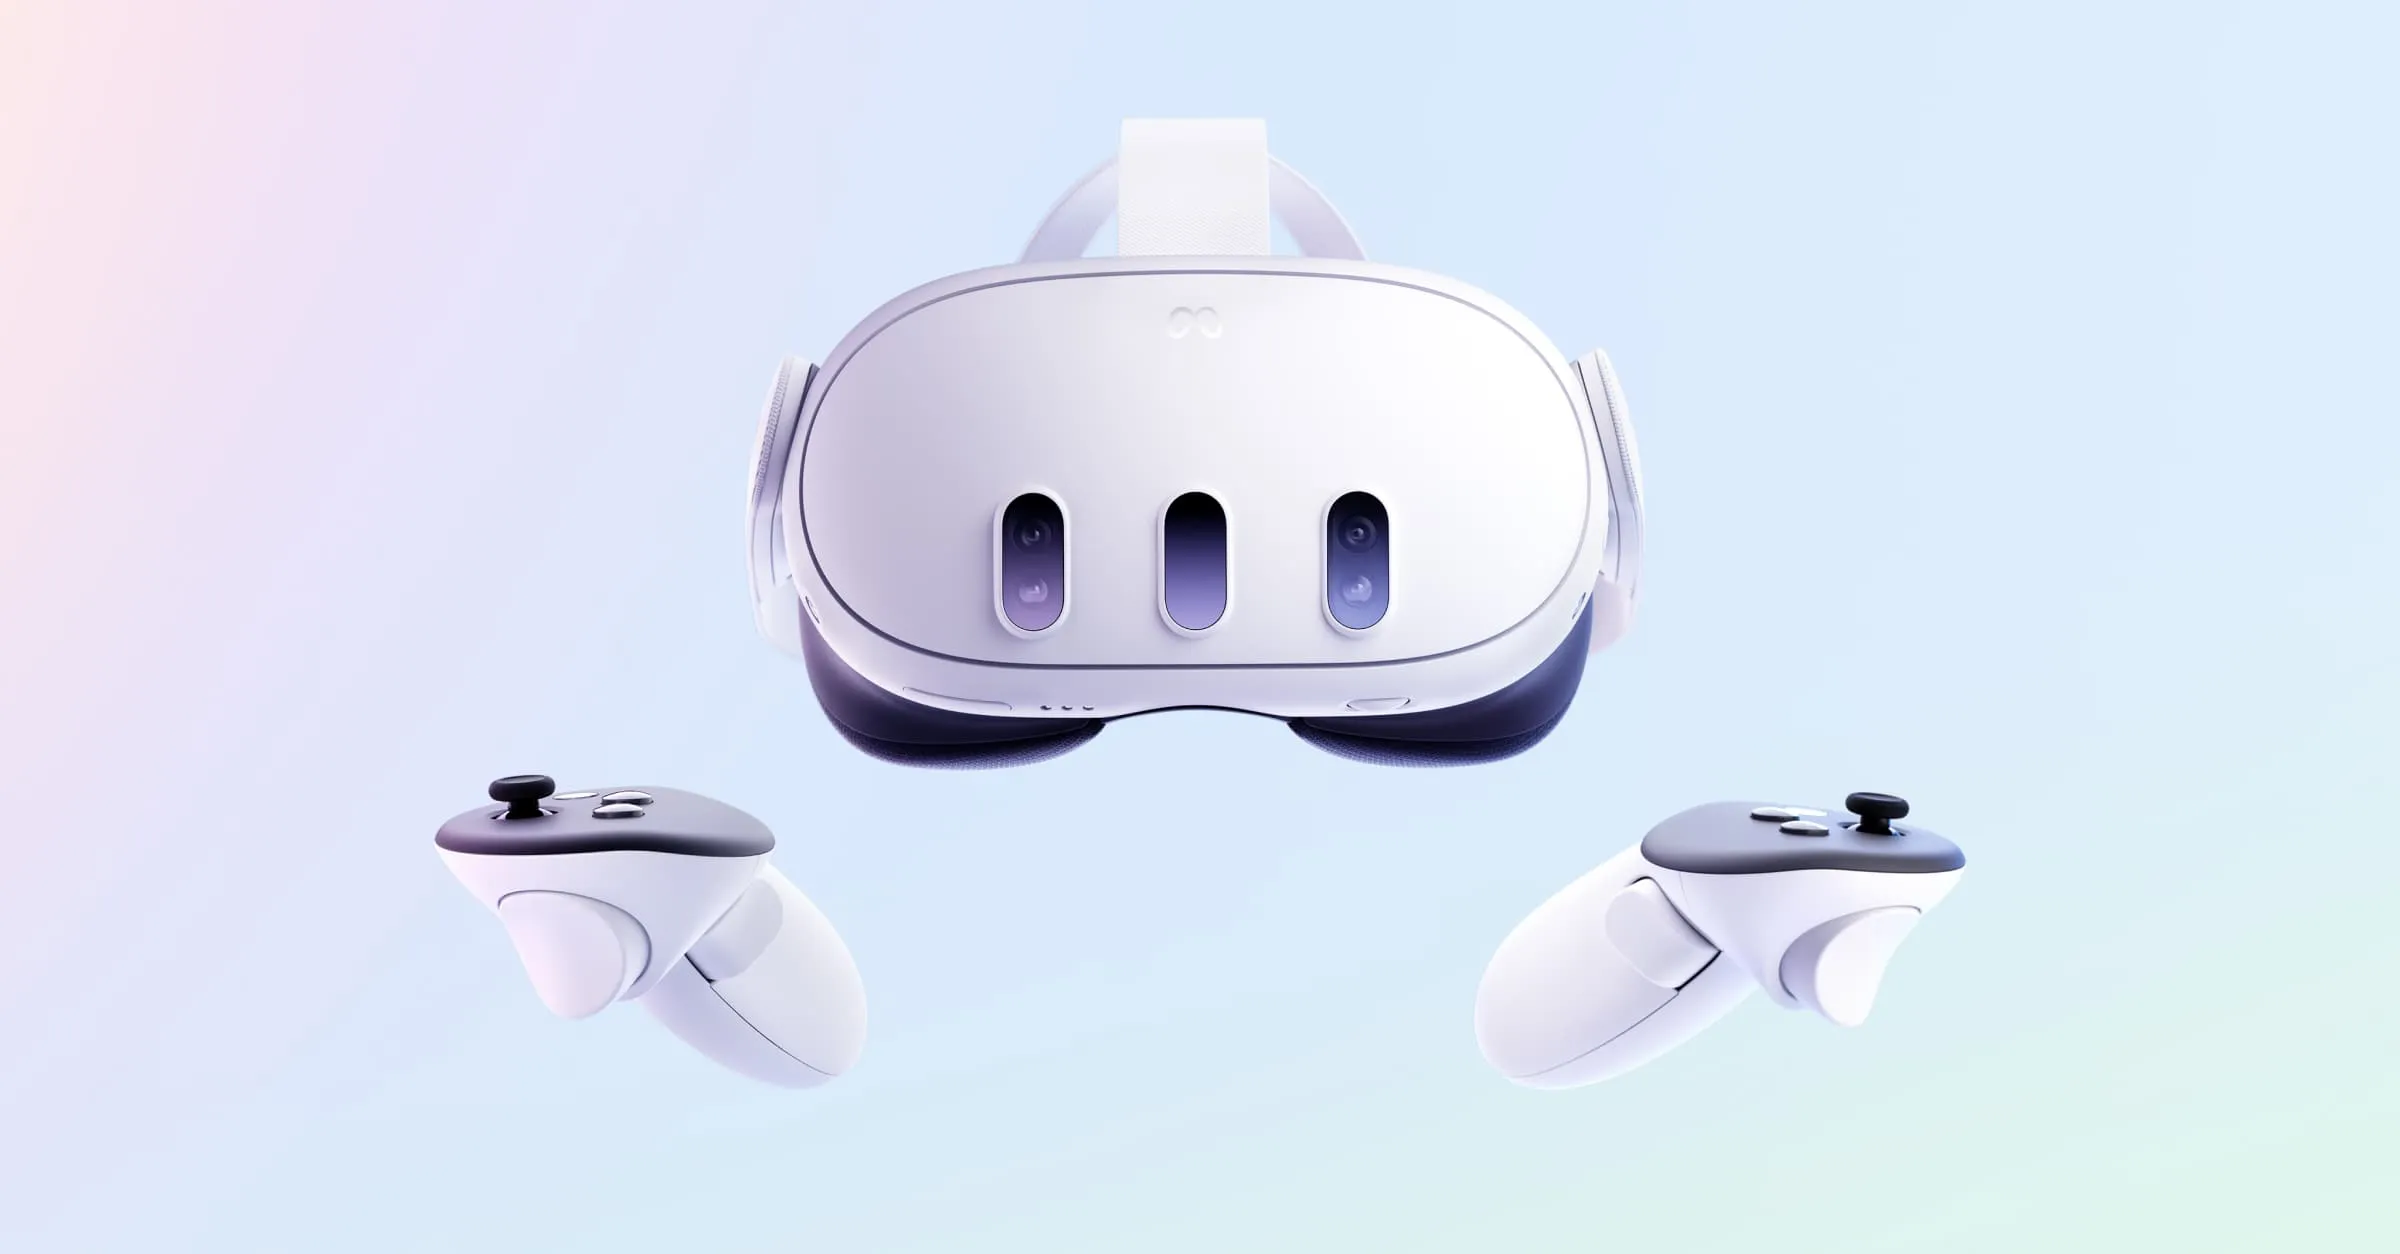
\includegraphics[width=0.8\textwidth]{NOVAthesisFiles/Images/papers/hmd-quest.png}
    \caption[Oculus Quest 3 and its Controllers]{The Oculus Quest 3 and its Controllers. The headset's frontal cameras and IMU(Inertial Measurement Unit) allow a wireless 
    \gls{6DOF} and gesture tracking system.}
    \label{fig:hmd-quest}
\end{figure}

Input devices also have their importance in user interactions with \glspl{VE}~\cite{Lee2020}, with these taking multiple forms.
Controllers are the most common within the \gls{VR} space~\cite{Anthes2016,Boletsis2022}, demonstrating similarities with the familiar 
video-game controllers with the inclusions of buttons for discrete input, and joysticks and triggers for continuous input. \gls{VR} controllers 
distinguish themselves from the video-game ones by including \gls{6DOF} tracking capabilities and by integrating gesture-recognizing sensors.

Other input devices range from Gesture Tracking devices, with data gloves as an example, to navigation devices, such as \glspl{ODT} 
and Zero-Friction Surfaces~\cite{Anthes2016,Nilsson2018}.

\subsection{Development of VR Applications and Environments}
\label{sec:vr-apps-environments}

Tools and technologies have emerged alongside the "second-wave" of \gls{VR} development~\cite{Anthes2016}, making \gls{VR} application development 
more accessible. Popular 3-D game engines, such as \textit{Unity}\footnote{Unity Documentation - \href{https://docs.unity3d.com/Manual/index.html}{https://docs.unity3d.com/Manual/index.html}, Last Access - Feb 2025} 
and \textit{Unreal Engine}\footnote{Unreal Engine Documentation - \href{https://docs.unrealengine.com/}{https://docs.unrealengine.com/}, Last Access - Feb 2025}, 
are examples of tools that support \gls{VR} development. These engines help developers streamline the process of creating \glspl{VE} and the interactions that occur 
within them, through the use of diverse plugins and libraries for XR development.

\textit{OpenXR}\footnote{OpenXR Main Page - \href{https://www.khronos.org/openxr/}{https://www.khronos.org/openxr/}, Last Access - Feb 2025} by 
\textit{Khronos Group} is an open, royalty-free standard for \gls{VR} and \gls{AR} applications. This standard defines a unified interface 
for developers to use when developing \gls{VR}/\gls{AR} applications, providing cross-platform compatibility between various \glspl{HMD}, 
so that low-level programming for these platforms is more accessible, since developers do not need to program the application according to 
each of the \glspl{SDK} from each platform.

Due to the availability of these tools, the scientific community has been using them to create \gls{VR} applications and environments \cite{Anthes2016}. 
This research is included in this group, as the \textit{Unity} game engine will be used along with \textit{OpenXR} plugins to develop the applications 
of our proposed solution.  

\subsection{Navigation of Virtual Environments}
\label{sec:navigation-in-ves}

Due to the immersive yet controlled nature of \gls{VR}, one of its effective applications involves the study of human navigation behavior 
~\cite{Feng2022}. This research belongs with those studies, thus it is relevant to have an overview on this matter, as well as understanding its 
nomenclature, which is the purpose of this section.

\textbf{Navigation} can be broken down into \textit{Motion} - its physical element - and \textit{Wayfinding} - its cognitive element 
~\cite{Eastgate2014}. The model constructed by Jul and Furnas~\cite{Jul1997}, as seen on Figure~\ref{fig:nav-model} is considered a relatively complete representation 
of how Navigation takes place, since it takes both these elements into consideration.

\textit{Wayfinding} involves no movement of any kind, and its primary purpose is to construct and keep a \textit{cognitive map}
~\cite{Langbehn2018}, also referred to as \textit{mental maps}, which, as the name suggests, is a mental representation of an environment. 
Although it may be instinctive to call it a "picture in our heads", studies have come to suggest that these cognitive representations 
are not strictly visual but also symbolic~\cite{Eastgate2014, Warren2019}. The quality of a \textit{cognitive map} is then dependent on the 
method in which the spatial knowledge is acquired, as results of accurate spatial orientation differs from understanding a map to navigating  
non-immersive \glspl{VE} (such as those of video-games on a screen) and immersive \glspl{VE}~\cite{Eastgate2014,Santos2009}. Even then these 
results can be inconclusive, as the properties of \glspl{VE} affect the intake of spatial knowledge.

\textit{Motion}, also referred as \textit{Locomotion} or \textit{Travel}, is the motor element of Navigation that allows the physical translation 
from one location to another~\cite{Santos2009}. The properties of motion have implications on the intake of spatial knowledge, as for instance, 
if locomotion in a \gls{VE} is discrete instead of continuous, users tend to have more difficulty in fully comprehending their 
surroundings~\cite{Langbehn2018}. This 
and other properties of locomotion are then going to be discussed in the following sections of \nameref{sec:vr-locomotion-techniques} and 
\nameref{sec:non-euclidean-space}.

\begin{figure}[t]
   \centering
   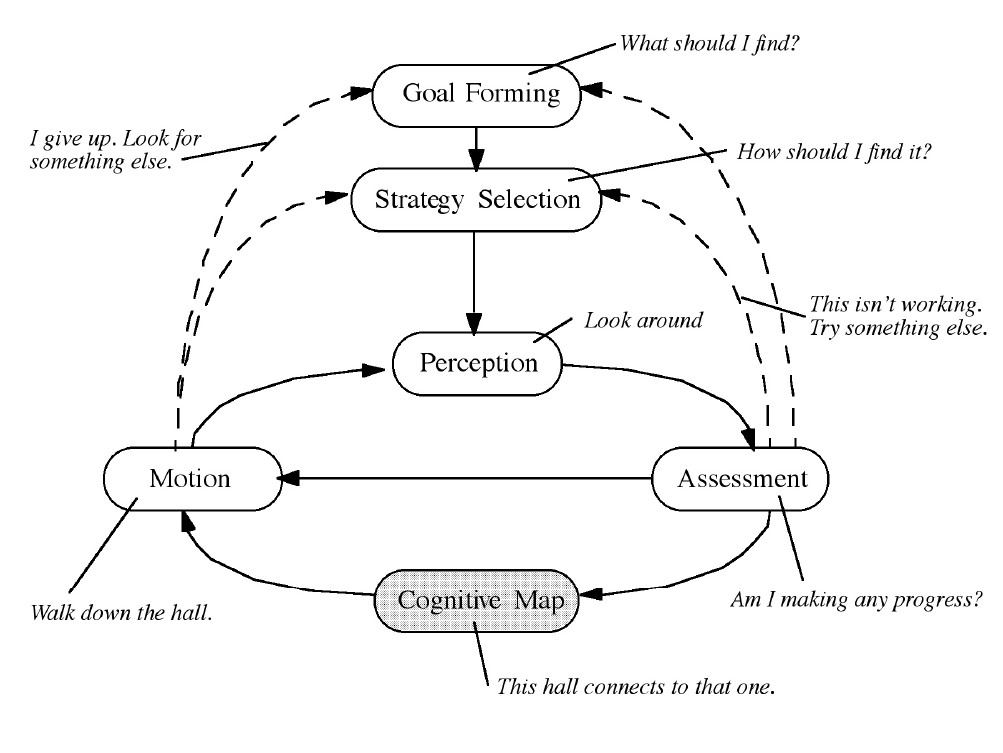
\includegraphics[width=0.75\textwidth]{NOVAthesisFiles/Images/papers/nav-model.png}
   \caption[Navigation Model by Jul and Furnas]{Model by Jul and Furnas that demonstrates the motor and cognitive elements of Navigation~\cite{Eastgate2014}.}
   \label{fig:nav-model}
\end{figure}

\section{VR Locomotion Techniques}
\label{sec:vr-locomotion-techniques}

Locomotion (also denoted as "active travel" or just "travel"~\cite{Langbehn2018}) - 
the act of moving from one location to another - is often considered one of the key aspects of \gls{VR} interaction~\cite{8255772}, 
as it permits navigation in \glspl{VE}~\cite{Boletsis2019}.

Throughout the advancements in \gls{VR} research and technology, multiple locomotion techniques have been developed, 
all with different characteristics, addressing different needs and use cases~\cite{Boletsis2022}. 
It is due to the diversity of these techniques that various taxonomies and classifications have been proposed,
throughout the years of \gls{VR} development~\cite{Boletsis2022}. 
The structure of this subsection is based on the typology of \gls{VR} Locomotion Techniques proposed by Boletsis et al.~\cite{Boletsis2022} 
as it encompasses most techniques according to the characteristics discussed in this section.

According to Boletsis et al.~\cite{Boletsis2022} locomotion techniques are distinguished by the type of interaction they require, 
the type of motion it produces and the type of \gls{VE} it is designed for, as seen in Figure~\ref{fig:vr-locomotion-typology}.
\begin{figure}[t]
    \centering
    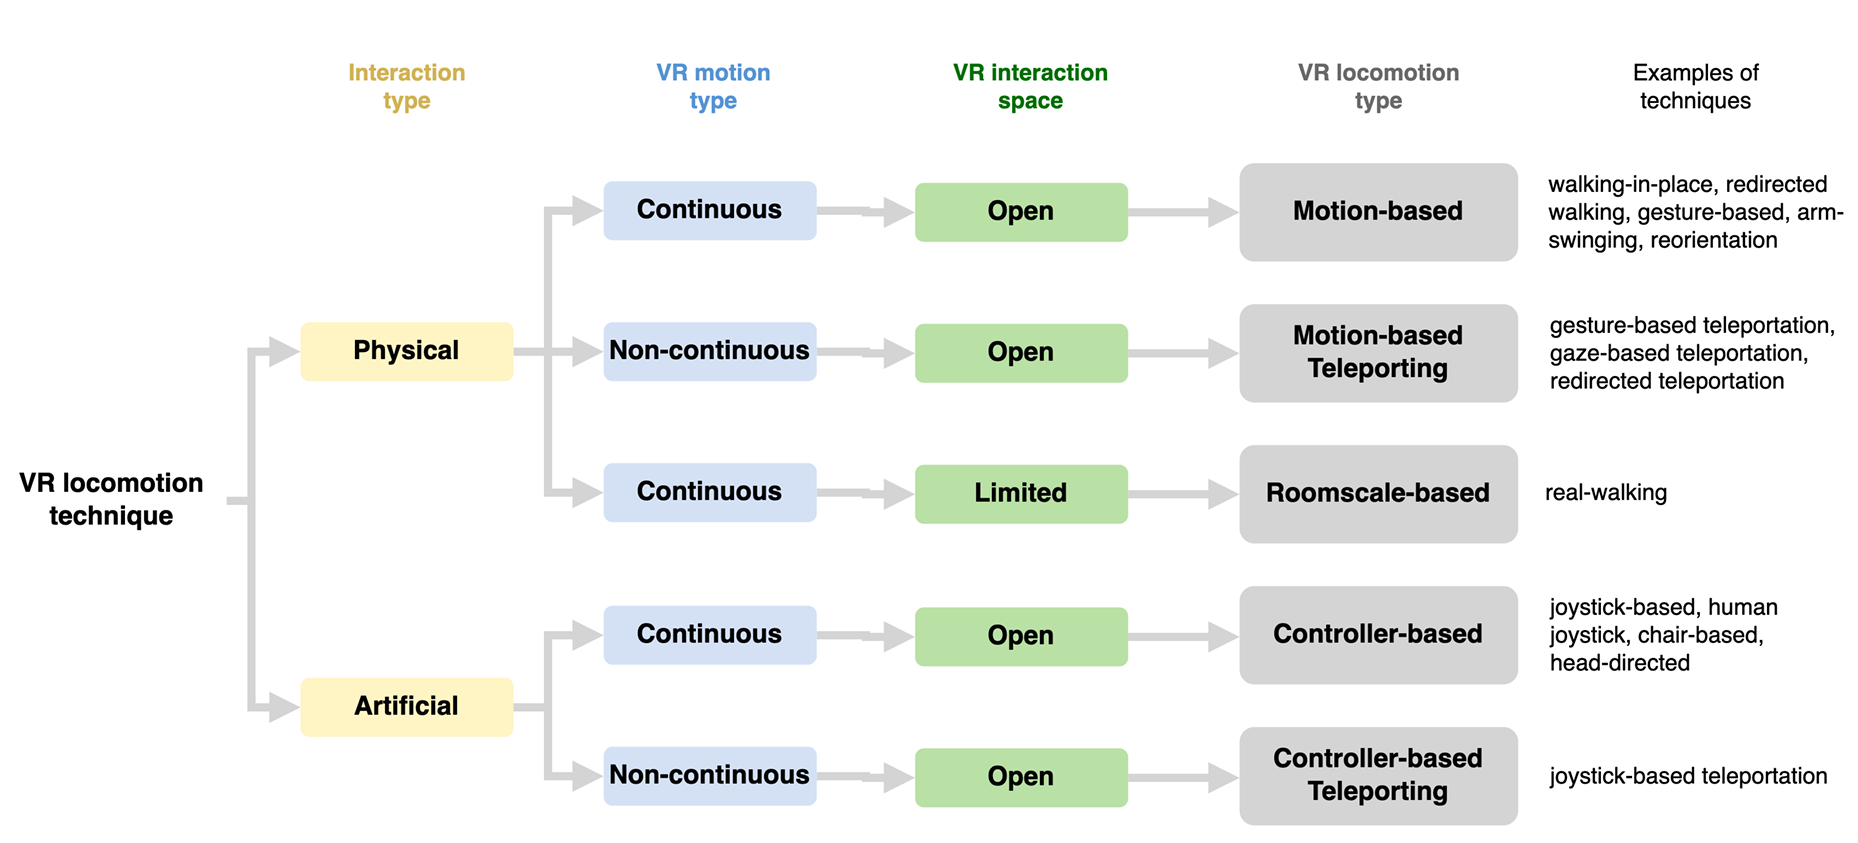
\includegraphics[width=\textwidth]{NOVAthesisFiles/Images/papers/vr-locomotion-typology.png}
    \caption[Typology of \gls{VR} locomotion techniques]{Typology of \gls{VR} locomotion techniques by Boletsis et al.~\cite{Boletsis2022}}
    \label{fig:vr-locomotion-typology}
\end{figure}

Regarding the interaction type, a locomotion technique can be "physical" - 
the input is based on physical movement - or "artificial" - utilizes input devices for direct \gls{VR} motion and navigation.
\gls{VR} motion types may be "continuous" - the transitions between positions is smooth and non-interrupting - 
or "non-continuous" - the transitions between positions are abrupt or instantaneous.
Finally, the \gls{VR} interaction space may be "open" - the \gls{VE} is larger than the tracking space being used - 
or "limited" - the physical environment constraints the size of the \gls{VE}.

Different sets of these characteristics define the different types of 
locomotion techniques that are to be discussed in the following sections. 
It is also important to note that these techniques may be used in combination with each other, 
i.e., a technique integrating two or more other techniques~\cite{Boletsis2022}.

\subsection{Controller-Based}
\label{sec:controller-based}


Controller-Based locomotion techniques are used in an open \gls{VR} interaction space, with continuous motion and require 
an artificial means of input, such as a controller or other similar input devices~\cite{Boletsis2017}.
Joystick-based locomotion is not only the most prevalent of this type of techniques, it is also one of the most used 
techniques in research~\cite{Boletsis2022}.

Joystick-Based locomotion can be described in the following manner: given a user in a \gls{VE} from a \gls{VR} application, 
the way that they navigate in said \gls{VE} is dependent on a joystick controller. The joystick rests in a neutral position until the user
applies force, changing its value in a certain axis, normally from -1 to 1 (see Figure~\ref{fig:vive-joystick}). The values registered 
on the horizontal and vertical axis will make the user continuously translate from one position to the next in the 
direction related to the user's gaze direction, i.e., if the user is looking in a certain direction and applies vertical of 1 
they will move in the yaw direction of their gaze at full speed~\cite{Coomer2018}.
\begin{figure}[t]
    \centering
    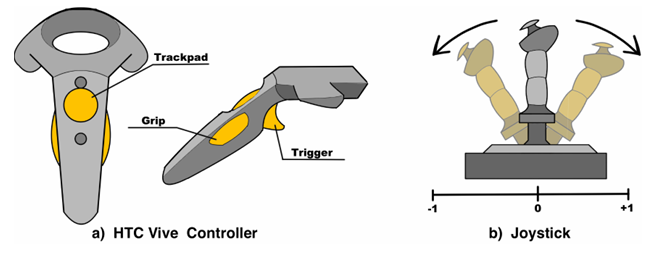
\includegraphics[width=0.75\textwidth]{NOVAthesisFiles/Images/papers/vive-joystick.png}
    \caption[Diagram of Vive Controller and Joystick]{Diagram of Vive Controller and Joystick~\cite{Coomer2018}}
    \label{fig:vive-joystick}
\end{figure}
The artificial means of creating input for movement makes joystick locomotion considered not physically demanding and a high ease-of-use 
technique, especially noticed in users who have prior experience with similar controllers~\cite{Nasiri2023}. This locomotion type also registers 
moderate-to-high levels of immersion when used, mostly due to the motion's uninterruptible nature~\cite{Boletsis2019}.

Though intuitive and not physically demanding, joystick locomotion has a caveat that pertains to the discomfort users might feel during motion. 
This locomotion type can create
motion sickness, due to the conflicting movement cues from user's proprioception, their vestibular sense and from their vision, as the user 
is physically stationary whilst they move in the \gls{VE}~\cite{Langbehn2018}. This is especially felt by inexperienced \gls{VR} users~\cite{Nasiri2023}.

\subsection{Teleportation}
\label{sec:teleportation}

Teleporting differs from Controller-Based locomotion techniques in that it is non-continuous, as, 
instead of moving continuously, users are teleported from one location to the next in an interrupted manner during their navigation~\cite{Boletsis2017}, 
and, similarly to \nameref{sec:controller-based}-Based locomotion, it is one of the most used locomotion techniques~\cite{Boletsis2022}.

When teleporting, a user dictates where they want to teleport to, usually by holding down some input button on a controller and pointing to
the pertained destination with said controller, releasing said input when the destination has been chosen. On release the user 
moves to the selected destination instantaneously (see Figure~\ref{fig:teleporting})~\cite{Coomer2018, Nasiri2023}.

\begin{figure}[b]
    \centering
    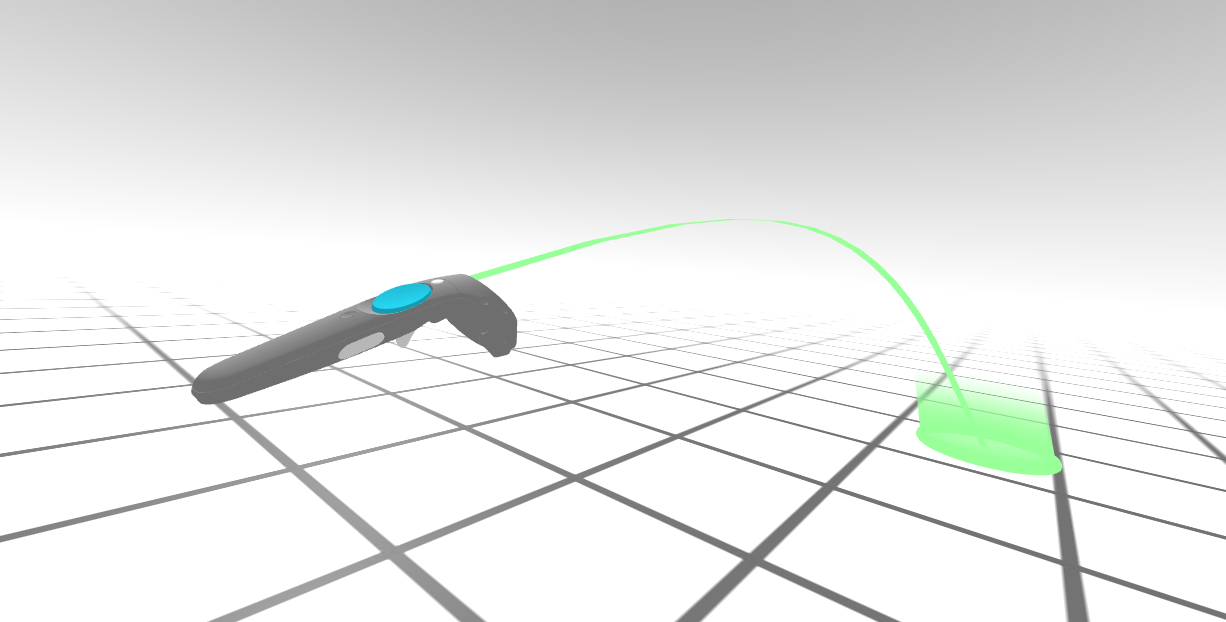
\includegraphics[width=0.6\textwidth]{NOVAthesisFiles/Images/papers/teleporting.png}
    \caption[Graphical Representation of Teleporting]{Graphical Representation of Teleporting\footnote{Aframe Teleport Component by Fernando Serrano - \href{https://aframe.io/blog/teleport-component/}{https://aframe.io/blog/teleport-component/} - Last Access: Feb 2025 } 
    }
    \label{fig:teleporting}
\end{figure}

The discontinuity of this locomotion method creates strengths and weaknesses. On the positive side, the discrete jumps prevent feelings of
cybersickness by not having a conflicting continuous motion occurring while the user is stationary~\cite{Boletsis2019, Nasiri2023}, 
and is generally more efficient at covering long distances~\cite{Coomer2018}. On the other hand the jumps can create some disorientation and
loss of immersion, as after teleporting the user takes more time to fully comprehend their surroundings~\cite{Langbehn2018}, exerting more
cognitive effort and in turn breaking the illusion of the \gls{VE}.

To mitigate this lack of immersion, studies tried to provide less artificial manners of performing teleportation. However, even with similar or 
slightly better results in regard to immersion, users still preferred using controllers rather than the purposed controller-free~\cite{Bozgeyikli2016}, 
and even hands-free teleportation techniques~\cite{Prithul2022}.

Even so, in various comparison studies, teleportation has been identified as a preferred locomotion method over other frequently used 
alternatives, mostly due to the lack of motion sickness and high ease-of-use~\cite{Boletsis2019, Langbehn2018}.

\subsection{Omnidirectional Treadmills}
\label{sec:omni-directional-treadmills}

As a type of locomotion techniques that require physical interaction for continuous motion in open \gls{VR} interaction spaces, 
Motion-Based techniques are rooted on physical movement for navigation in a \gls{VE}~\cite{Boletsis2017}, which poses the
question: How can a user physically navigate a \gls{VE} larger than their physical environment without reaching the limits 
of their available space?

According to Nilsson et al.~\cite{Nilsson2018}, it is possible to identify yet another three subtypes of Motion-Based 
locomotion techniques, all of which try to solve this problem, with these being Repositioning Systems, Proxy Gestures and 
Redirected Walking.

Repositioning Systems refer to input devices that try to counter-act forward motion when users walk, essentially keeping them in place, 
ranging from more devices with a more "active" approach to the repositioning, such as treadmills to more "passive" options, such as friction-free
platforms Figure~\ref{fig:repo-systems}.

\begin{figure}[b]
    \centering
    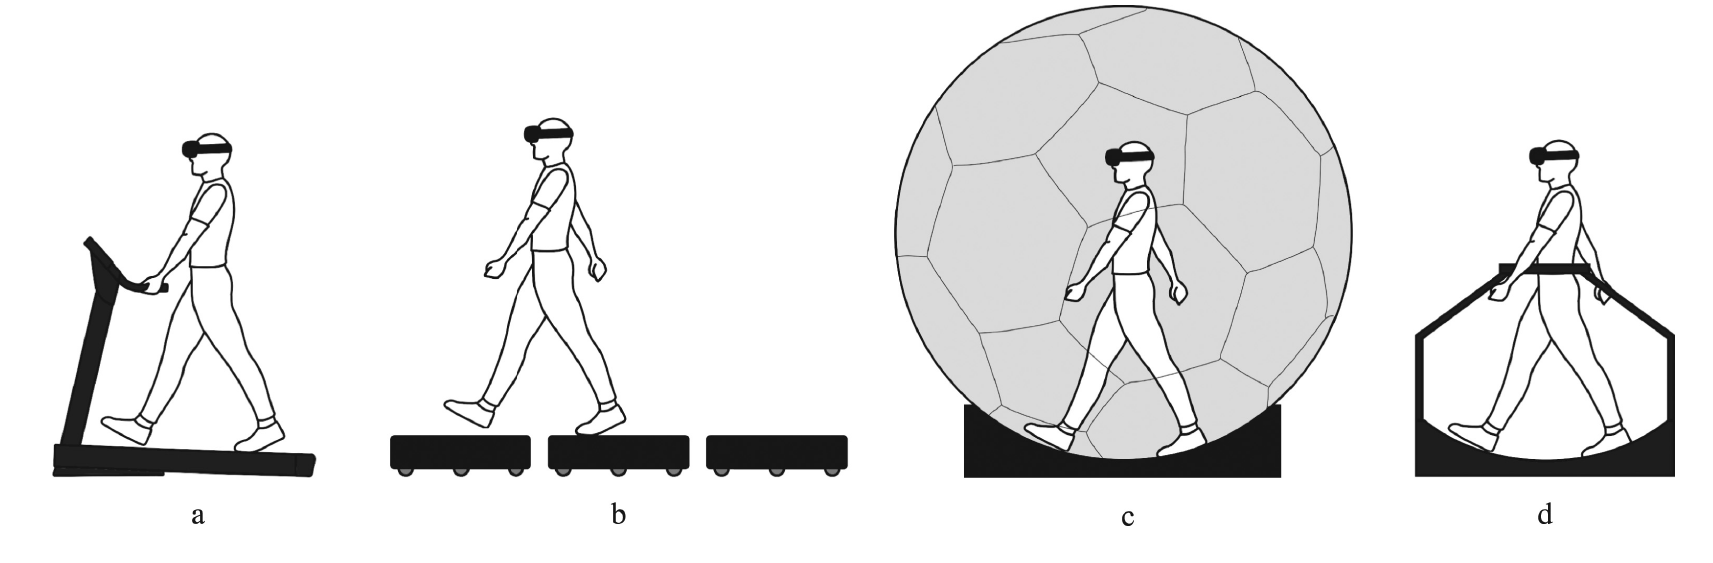
\includegraphics[width=\textwidth]{NOVAthesisFiles/Images/papers/repo-systems.png}
    \caption[Common Re-Positional Systems]{Four examples of re-positional systems: (a) Traditional Linear Treadmill, (b) motorized floor tiles,
    (c) a human-sized hamster ball, and (d) a friction-free platform.~\cite{Nilsson2018}}
    \label{fig:repo-systems}
\end{figure}


One of the most common Repositioning Systems are Omnidirectional Treadmills - devices that sense the direction of steps whilst a user is
walking in a 360 degree space, maintaining the user at the center of their available space, translating the users steps as movement in the \gls{VE}.
User studies seem to indicate that the motion caused, although not reaching quite exactly the feeling of real walking (with some users indicating a 
feeling more similar to running or skating rather than walking), this locomotion method evokes high levels of presence, similar to natural 
walking locomotion methods~\cite{Syamil2024}.

However, despite taking an almost accurate walking motion as input, offering high levels of immersion and providing a promising solution 
for the physical limitations of walking in a constricted space, these devices are often expensive and tend to be difficult to operate~\cite{Cherni2020}.
In addition, performing quick turns or side-steps may cause users to lose balance~\cite{Nilsson2018} and more natural walking techniques 
such as the latter discussed \nameref{sec:redirected-walking} are preferred by users~\cite{Syamil2024}. 

\subsection{Walking-In-Place and Arm-Swinging}
\label{sec:wip-and-as}

Proxy Gestures techniques, contrarily to Repositioning Systems, such as the \nameref{sec:omni-directional-treadmills}, offer inexpensive 
and easy-to-learn solutions to the problem caused by physical constraints during Motion-Based locomotion techniques~\cite{Nilsson2018}. 
Locomotion in these techniques is based on gestures that emulate walking motions, keeping users moving their limbs, but 
stationary at the same time.

Walking-In-Place is the most common of these techniques~\cite{Boletsis2019,Nilsson2018}. To emulate walking, users perform a 
gesture comparable to "marching on the spot" in order to move in the direction they are facing, sometimes relying on sensors for 
detecting leg movements~\cite{Cherni2020}, yet the detection can recur solely to \glspl{HMD}~\cite{Lee2018} (Figure~\ref{fig:wip}).

\begin{figure}[b]
    \centering
    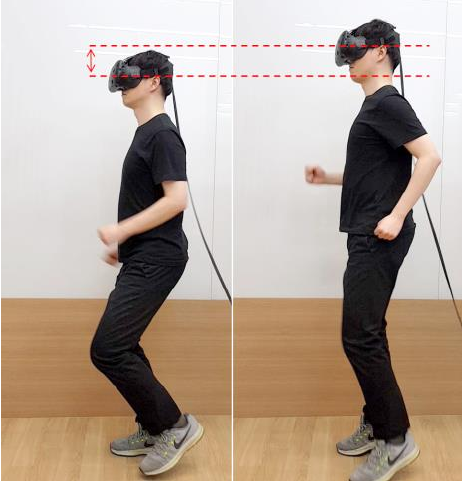
\includegraphics[width=0.4\textwidth]{NOVAthesisFiles/Images/papers/wip.png}
    \caption[Walk-in-Place Tracking Example]{A visualization of how Walk-In-Place may be detected by an \gls{HMD}, through the variance of its position.~\cite{Lee2018}}
    \label{fig:wip}
\end{figure}

Although it might sound counter-intuitive for simulating physical walking, Arm-Swinging is a technique that switches the 
motion performed by users from the lower body to the upper body. In this technique users swing their arms back and forth interchangeably, 
to move in the direction they are facing. The objective is to perform a gesture comparable to how humans naturally swing their 
arms when they walk, with arm movements being detected either by armband-like sensors~\cite{Cherni2020}, or just by 
controllers that users hold in their hands~\cite{Coomer2018}.

The fact that both these techniques have the capability to only rely on \glspl{HMD} and their associated 
Controllers makes them more accessible, easier to use and thus a more prevalent technique 
for common users~\cite{Nilsson2018}. Additionally, the motion-based input provides a more appropriate proprioceptive feedback 
similar to real walking than \nameref{sec:controller-based} and \nameref{sec:teleportation} 
techniques and hence usually grade higher in immersion ratings~\cite{Boletsis2019}. 

Despite this, these techniques present some caveats. Walking-In-Place can be physically demanding and potentially 
induces motion sickness after prolonged use~\cite{Boletsis2019,Cherni2020}, making it not the best solution for use-cases 
in which users have to navigate an extensive \gls{VE}. Arm-Swinging, although not in the same magnitude, is also limited by this 
weak point~\cite{Coomer2018}, but it is additionally limited by the fact that users cannot use their arms for interaction 
while moving~\cite{Nilsson2018}. 

\subsection{Redirected Walking}
\label{sec:redirected-walking}

Motion during navigation in \gls{VR} is an added value to immersion. The previously mentioned techniques - \nameref{sec:omni-directional-treadmills},  
\nameref{sec:wip-and-as} - proved this, since they are regarded as high immersion techniques compared to techniques with artificial means of 
input (\nameref{sec:controller-based} and \nameref{sec:teleportation}), due to their reliance on gestures that simulate walking~\cite{Nasiri2023}.
Additionally, Motion-Based techniques also tend to score higher in spatial orientation/awareness, compared to artificial means~\cite{Cherni2020,Coomer2018}.
Even so, users tend to prefer using \gls{RDW} over the other motion-based techniques~\cite{Langbehn2018, Syamil2024}.

\gls{RDW} is not a particular technique, but rather an umbrella term for all techniques that allow users to physically walk in a 
\gls{VE} by controlling their path in ways that keep them from reaching the edges of their available physical space~\cite{Nilsson2018}. 
Despite the multitude of possible implementations, \gls{RDW} aims to follow 4 criteria: \textbf{Imperceptibility} - users should be as less aware 
as possible of the redirection taking place - \textbf{Safety} - users should feel as safe as possible from reaching the boundaries of their 
available physical space - \textbf{Generality} - the correct functionality of the technique should be as independent as possible from the physical 
environments in which they might be used - and \textbf{Absence of Unwanted Side Effects} - the technique should aim to be devoid of 
side effects as those of cybersickness and disorientation~\cite{8255772}.

Literature on this topic has recognized two common types of redirection strategies adopted by these techniques~\cite{8255772, Nilsson2018}:
\begin{itemize}
    \item \textbf{Perspective Manipulation} - 
    RDW techniques that steer users away from the edges of their tracking space by manipulating the mapping between the real 
    and virtual movements performed by users. Manipulation is accomplished by applying repositioning and orientational transformations, such as gains to 
    the users translational and rotational movements
    i.e. if a gain of 2.0 is applied to the user's 
    forward translation, then they will travel twice as fast in that forward motion in the \gls{VE}
    
    \item \textbf{Environment Manipulation} - 
    These techniques rely on the layout and characteristics of the\gls{VE} in order to accomplish redirection. This is done by either 
    building a \gls{VE} with a pretended path or by changing the \gls{VE}'s properties whilst the user is navigating it, in order to change 
    the routes taken by users, with the purpose of keeping them away from the limits of their available space.
\end{itemize}

\subsection{Overt and Subtle Redirection}
\label{sec:ov-sub-redirection}

To further categorize these techniques, Suma et al.~\cite{6180877} purpose a taxonomy of techniques (observable in Figure~\ref{fig:rdw-taxonomy}) 
according to whether these 
are \textbf{Repositioning Techniques} - techniques that compress the \gls{VE} by manipulating the correspondence between points in the real 
and virtual environments - and \textbf{Reorientation Techniques} - techniques that attempt to rotate the facing direction of users away from 
the edges of their tracking space. These techniques can then be \textbf{Overt} - easily noticed by users - or \textbf{Subtle} - changes are 
hidden from users - and either \textbf{Continuous} - the changes are slowly applied - or \textbf{Discrete} - changes are immediate.
\begin{figure}[b]
    \centering
    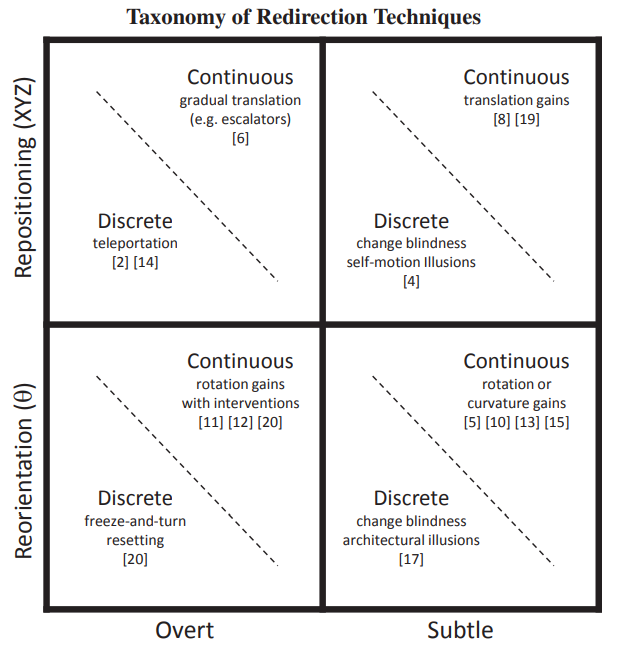
\includegraphics[width=0.45\textwidth]{NOVAthesisFiles/Images/papers/rdw-taxonomy.png}
    \caption[Taxonomy of Redirection Techniques]{Taxonomy of redirection techniques for supporting natural
    walking through immersive \glspl{VE}. The vertical axis
    distinguishes how the technique is applied in the environment. The
    horizontal axis provides a ranking in terms of notability to the user.
    The division in cells represents distinct implementation strategies for
    each type of technique.~\cite{6180877}}
    \label{fig:rdw-taxonomy}
\end{figure}

\textbf{Subtle Continuous Repositioning} and \textbf{Reorientation} techniques are associated with the use of Translational and 
Rotational Gains, respectively, and these could be considered the most prevalent techniques of the mentioned 
Perspective Manipulation strategy for redirection~\cite{Nilsson2018}. These gains compress the \gls{VE} by deliberately altering the 
mapping between movements in the physical and virtual spaces (Figure~\ref{fig:rdw-gains}). 
Translation Gains scale the steps users take, whilst Curvature 
Gains are a continuous small rotations applied while the user is walking forwards, creating the possibility for users to walk infinitely 
along a virtual path while walking in circles in their tracking space. Bending Gains are another type of gain that works similarly to 
Curvature Gains, but these are used in already curved virtual paths. Both Curvature and Bending Gains require either \textit{a priori} 
knowledge or a good prediction method of the path users take in the \gls{VE}~\cite{8255772}.

Most of the techniques in this taxonomy are associated with a Perspective Manipulation strategy. However, 
\textbf{Subtle Discrete Reorientation} techniques do directly alter the \gls{VE} making them accurately follow the
Environment Manipulation strategy. Change blindness redirection~\cite{5759455} serves as an example of how a technique 
with this characteristic might be used, as it discreetly makes changes to the environment outside users' \gls{FOV}, leading them to take different 
paths without breaking immersion.

With the given nomenclature, \textbf{Subtle Discrete Repositioning} might seem counter-intuitive, for how can a \gls{VR} application 
make discrete jumps in positions users take without their awareness? Bruder et al.~\cite{Bruder2011} purposed a solution by creating visual 
optic flow effects, reminiscent of filters or tunnel vision, to mask the discrete jumps in the users position. User studies performed 
with the implementation of this technique revealed that users were not able to discern the difference between real and virtual movements 
while influenced by the technique, allowing the redirection to be more imperceptible.

\begin{figure}[t]
    \centering
    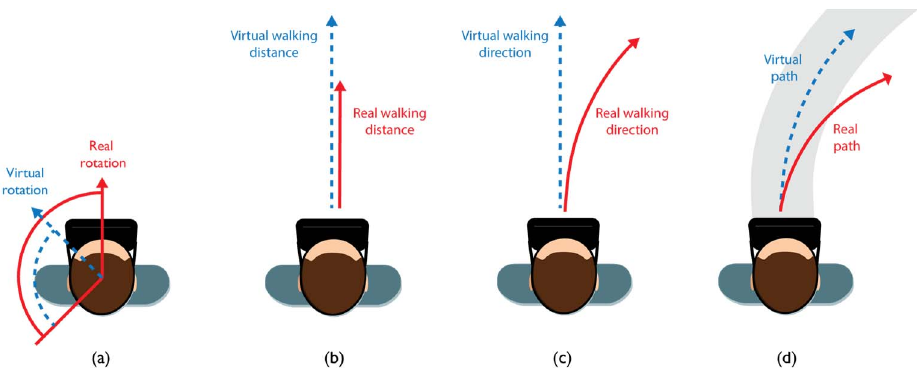
\includegraphics[width=0.75\textwidth]{NOVAthesisFiles/Images/papers/rdw-gains.png}
    \caption[Illustration of types of redirection gains]{Illustration of four types of gains used to manipulate the mapping between the real
    and virtual movements: (a) rotation gains (user stationary), (b) translation gains (user moving
    forward), (c) curvature gains (user moving forward), and (d) bending gains (user moving on a
    curve).~\cite{8255772}}
    \label{fig:rdw-gains}
\end{figure}

As mentioned, \gls{RDW} techniques should aim to be as unnoticeable as possible~\cite{8255772}, but overt techniques prove valuable in 
limiting conditions to assert that the technique is safe for use. \textbf{Overt Discrete Reorientation} techniques are associated with 
techniques used to redirect users to the available space when they are near of its limits. Freeze-and-turn is an exemplary 
"failsafe" emergency technique~\cite{Williams2007}. When a user is nearing the edge of 
their tracking space, the display on the users' \glspl{HMD} freezes and prompts them that 
a reset is required. Once the user has completed a 180-degree turn, the display resumes. 
Even if the redirection is easily noticeable, Safety can be prioritized over 
Imperceptibility for extreme cases such as these.

\begin{figure}[t]
    \centering
    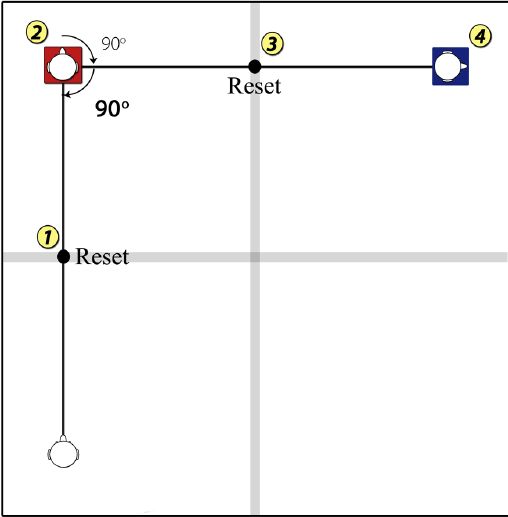
\includegraphics[width=0.5\textwidth]{NOVAthesisFiles/Images/papers/freeze-n-turn.png}
    \caption[Freeze-and-Turn use-case example]{Illustration of one of the case studies by Williams et al.~\cite{Williams2007} when testing the Freeze-and-Turn technique. 
    In a subdivided virtual space, in this case 4 times larger than the available tracking space, whenever a user finds themselves at the limit of 
    the tracking space, they are forced to "reset", by doing a 180º turn while the \gls{VE} is frozen. 
    The resulting condition is that users keep walking in the direction 
    they were heading in the \gls{VE} but return to their available space in their tracking space.}
    \label{fig:rdw-gains}
\end{figure}

\textbf{Overt Continuous Reorientation} techniques are then comparable to the previously mentioned type of technique. The difference lies 
in the fact that when the system is resetting, the display does not freeze, as when the user is prompted to turn 180 degrees, their movements 
are being translated as a full 360-degree turn in the \gls{VE}, allowing them to proceed their virtual path without reaching the edges of 
their tracking space~\cite{Williams2007}.

\textbf{Overt Discrete Repositioning} relies simply on teleporting the user from one position to the next, which may be disorienting if 
users are not given enough context and are not expecting the instantaneous change in space. This is mitigated through the use of portals, 
making the transition more deliberate and potentially a more immersive experience~\cite{6180877}. This serves as an example that 
overt techniques do not necessarily severely reduce feelings of presence in a \gls{VE}, if there is a context that justifies the overtness. 

\textbf{Overt Continuous Repositioning} techniques simply translate the virtual environment about the user's position continuously, in order 
to achieve repositioning. This then allows the user to walk on areas in the virtual environment that were not previously
accessible within the confines of the physical workspace. To minimize the jarring sensations these techniques may feel, they can be coupled 
with the use of known metaphors associated with motion such as escalators, elevators and vehicles~\cite{6180877}.

It is important to note that techniques may incorporate more than one of the mentioned strategies and types of techniques. The work by 
Rebelo et al.~\cite{Rebelo2024} is an example of this, as the developed techniques rely on the use of portals, alterations in
structure of the \gls{VE} and translation gains, in order to permit the navigation of an extensive \gls{VE} in a room-scale physical space.

It is also relevant to note that \gls{RDW} techniques present caveats. These techniques typically need larger physical environments in order to be 
imperceptible~\cite{Langbehn2018}, since smaller tracking spaces imply the need for higher value gains and gains need to stay below detection 
thresholds to remain imperceptible, and thus more immersive~\cite{Grechkin2016}. Minimum room sizes and the mentioned gain thresholds are dependent on 
the techniques being used and remains a challenge for \gls{RDW} research.~\cite{Cherni2020, 8255772}. 

Techniques similar to Telewalk~\cite{Rietzler2020} directly address this limitation, 
as this technique aims to be a locomotion approach that permits navigation in VR in a more natural way to increase presence and immersion, in 
spaces as small as 3x3 meters. It relies on using intentionally overt Rotational and Translational Gains, with the addition of head-based direction 
control and visual indicators to help redirect users into an optimal path, as seen in Figure~\ref{fig:rdw-telewalk}. The user study conducted 
by Rietzler et al.~\cite{Rietzler2020} compared Telewalk with \nameref{sec:teleportation}, since, as mentioned previously, the latter is also highly 
optimal for use-cases in which the tracking space is reduced. Telewalk did result in stronger feelings of presence and immersion and was 
seen as more natural than Teleportation, mostly accomplishing its purpose, yet users were evenly divided in terms of preference between the two 
techniques. This was mostly due to an unwanted side effect created by the overtness of the technique, which leads to the next limitation of 
\gls{RDW}.

\begin{figure}[b]
    \centering
    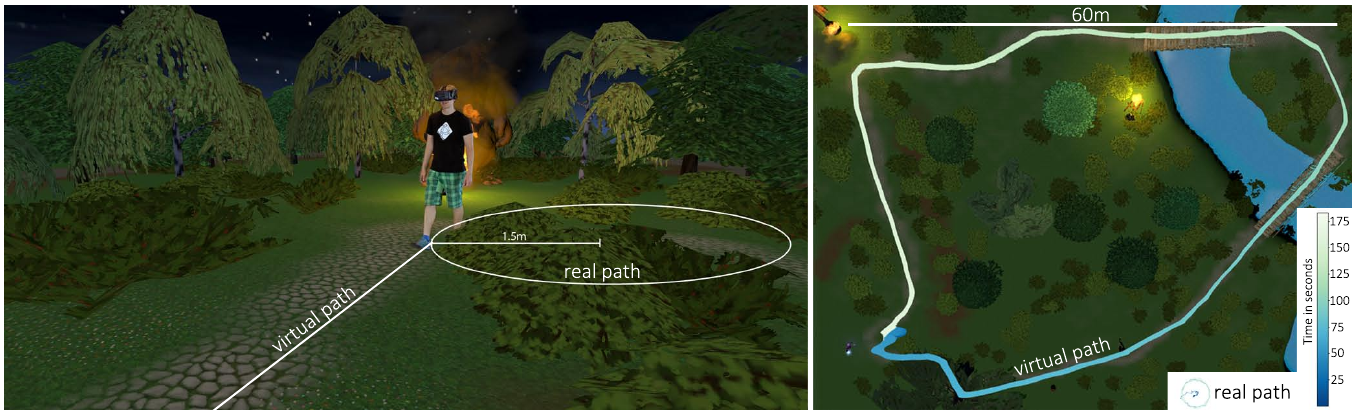
\includegraphics[width=\textwidth]{NOVAthesisFiles/Images/papers/rdw-telewalk.png}
    \caption[Illustration of Telewalk]{Telewalk: The combination of perceivable curvature and translation gains along with a head based camera
    control allows compressing any virtual space to a pre-defined real world radius (in this case 1.5m). (Left) illustration of walking paths
    and (right) plots of the virtual and real path walked in its study application.~\cite{Rietzler2020}}
    \label{fig:rdw-telewalk}
\end{figure}

\gls{RDW} techniques that create a large mismatch between real and perceived motion by using high translational gains 
can cause \gls{VR} sickness~\cite{Gemert2024}, as well as an increased cognitive load, particularly when overt redirection techniques 
are applied~\cite{8255772}. The effects vary depending on user characteristics, hardware, and gain configurations, thus 
an exact relationship between \gls{VR} sickness and \gls{RDW} remains unclear and a challenge in \gls{VR} research~\cite{Gemert2024, Grechkin2016}.

This is one of the challenges to be tackled in this research. After exploring the literature of Locomotion techniques, 
it is safe to say that \gls{RDW} techniques provide better levels of immersion and presence in the navigation of a \gls{VE}. It is, however, 
limited by the mentioned weak points, but, due to the diverse possibilities of implementations this type of locomotion techniques allows, 
alternatives that mitigate the problems created by these limitations can still be explored and refined. Thus, the accomplishing of this 
research's objectives involve the use of the mentioned strategies and techniques of \gls{RDW}.


\subsection{Comparing Techniques}
\label{sec:loc-summary}

Having an overview of the literature on \gls{VR} locomotion techniques allows for a clearer comprehension of the problem at hand. The objective of this section 
is to review the mentioned techniques and compare them, connecting their advantageous and disadvantageous characteristics (Table~\ref{table:locomotion-techniques})
to the best use-cases these techniques are optimal for, in search of conclusions that are valuable for addressing this problem.

\begin{longtable}
    {>{\hspace{0pt}}m{0.2\linewidth}>{\hspace{0pt}}m{0.35\linewidth}>{\hspace{0pt}}m{0.35\linewidth}}
    \caption{Summary of the explored Locomotion Techniques}\\
    \label{table:locomotion-techniques}\\
    \hline
    \textbf{Technique}          & \textbf{Advantages}                                                             & \textbf{Disadvantages} \\  
    \hline
    \endfirsthead 
    \hline
    Joystick-Based              & Intuitive; Easy to use; \par{} Moderate Immersion                       & Can cause motion sickness due to conflicting sensory cues                \\ 
    \hline
    Teleportation               & Prevents motion sickness; \par{} Efficient for covering long \par{} distances & Reduces immersion; Increases disorientation; Disrupts spatial awareness       \\ 
    \hline
    Omnidirectional Treadmills & High immersion; Realistic \par{} motion simulation                      & Expensive; Complex setup; Safety issues       \\ 
    \hline
    Walking-In-Place            & Affordable; Immersive; Minimal hardware requirements             & Physically demanding; Less natural than walking; Potential for motion sickness with prolonged use      \\ 
    \hline
    Arm-Swinging                & Accessible; Immersive; Minimal hardware requirements            & Limits hand use for interactions; Less natural than leg movements     \\ 
    \hline
    Redirected Walking (RDW)    & Highly immersive;\par{} Supports natural walking                      & Most techniques require larger physical spaces; High gain values can cause VR sickness         \\  
    \hline
\end{longtable}


After revising the studies made on this matter, it is possible to conclude that Continuity provide higher levels of presence in the \gls{VE}, 
since discreet jumps between locations lead to disorientation and unrealistic~\cite{Boletsis2019, Nasiri2023}. 
It is for this reason that, from the mentioned techniques, Teleporting was often considered the least immersive, 
despite its efficiency and user preference~\cite{Coomer2018}.
Motion-based implementations of this technique, such as 
Point-and-Teleport, however, have mitigated this~\cite{Bozgeyikli2016}, which supports the next conclusion.

Locomotion techniques reliant on artificial means of input, such as controllers, are less suited 
for providing high levels of presence in a \gls{VE}, compared to motion-based techniques. 
The lack of the appropriate proprioception feelings during navigation hinders 
immersion and may also result in cybersickness if the motion in the \gls{VE} is continuous~\cite{Langbehn2018, Nasiri2023}. 
Motion-based techniques, on the other hand, support higher feelings of presence, at the cost of ease-of-use 
~\cite{Boletsis2019, Cherni2020, 8255772, Nilsson2018, Syamil2024}. 

With the explored literature it is also possible to conclude that the more a Motion-Based technique resembles real walking the better it grades 
in immersion levels~\cite{Syamil2024}. An identified problem created by these techniques is the lack of physical space to map a walkable extensive 
\gls{VE}~\cite{Cherni2020, 8255772, Nilsson2018}. Walk-In-Place and Arm-Swinging present accessible solutions to
this problem, yet their representations of walking are not the most accurate~\cite{Cherni2020, Nilsson2018}. 
\glspl{ODT} provide a more similar feeling to natural walking (even if not perfect), 
but are not suited for use-cases in which the more complex set-up is to be avoided~\cite{Cherni2020,Syamil2024}. 
\gls{RDW} techniques resort to actual Natural Walking for locomotion, scoring high in immersion, yet this 
varies with the type of redirection being applied. As seen in the \nameref{sec:redirected-walking} section, these techniques can employ 
different types of redirection, and some of these are more overt than others~\cite{8255772, 6180877}. 
Imperceptibility seems to be the key aspect of a redirection technique that strengthens feelings of presence created 
by the naturalness of walking. 

From these conclusions \gls{RDW} proves to be the best route for this research, as its applicability is extensive and highly variable, and is the 
most suited for \gls{VR} applications that prioritize high immersion. Our implementation then needs to resort to redirection techniques that focus on maximizing 
the feelings of natural motion, and mitigate the overtness of the techniques.

\section{Non-Euclidean Spaces in VR}
\label{sec:non-euclidean-space}

As discussed in the \nameref{sec:navigation-in-ves} section, navigation employs mental effort, mainly through the 
act of intake and keeping of spatial information, which is supported by the use of the denominated cognitive/mental maps~\cite{Eastgate2014}. 
Being a mental representation of spatial data, its understanding is quite limited, although it is arguably instinctive to call it a 
"picture in our heads", yet studies as those of William Warren~\cite{Warren2019} reveal that this is inaccurate.

The experimental biology study done by Warren~\cite{Warren2019} defies navigation assumptions, by exploring Non-Euclidean spaces in \gls{VR}. 
Our perception of the real world is bound to the rules of 3 Dimensional Euclidean Geometry, and thus Non-Euclidean Spaces refer to spaces 
in which these rules are altered or do not apply, being then bound to a Non-Euclidean Geometry. This section's purpose is to explore 
two varieties of Non-Euclidean Spaces and their use in \gls{VR}: \nameref{sec:impossible-spaces}, which modify the geometric rules of distance, 
and \nameref{sec:hyperbolic-spaces}, which alter the Euclidean Parallel Postulate - given a line and a point not on that line, 
only one parallel line can be drawn through the point~\cite{Pisani2019}.

If one was to store spatial knowledge onto a Euclidean mental map, it would be conclusive that traversing a Non-Euclidean Space would prove to be 
disorienting, yet Warren's study proves the contrary~\cite{Warren2019}. In this \gls{VR} experiment, two groups of users had to traverse a maze, yet one group traversed the maze normally
whilst the other traversed a maze with the inclusion of invisible wormholes that seamlessly transported them from one position to another creating
a Non-Euclidean Impossible space, as seen in Figure~\ref{fig:warrens-mazes}. The mazes contained objects and the two tasks of the study  
consisted on firstly finding the objects and the routes between them, and then participants were asked to go one object to another in the shortest 
route possible without the mazes' structures, 
relying only on their spatial knowledge. The results on Figures \ref{fig:warrens-mazes} and \ref{fig:warrens-mazes-paths} show that 
the participants of the Non-Euclidean maze revealed a clear bias towards the use of the wormholes. Warren states that these results are in agreement 
with his hypothesis that spatial knowledge is represented as Cognitive Graphs, rather than Cognitive Maps, since despite the irregularities 
caused by the wormholes, participants consistently relied on local metric cues and graph-like relational behavior. 


\begin{figure}[t]
    \centering
    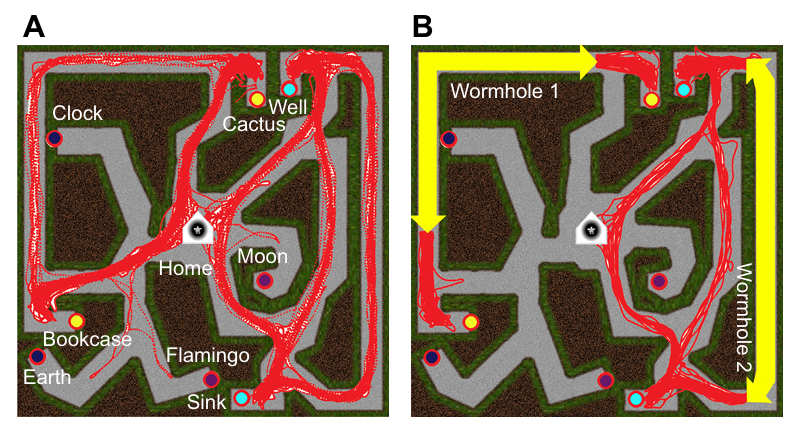
\includegraphics[width=0.45\textwidth]{NOVAthesisFiles/Images/papers/warrens-mazes.png}
    \caption[Map of the traversed mazes in the study by William Warren]{Traversed mazes in study by William Warren, 
    where A is the "normal" Euclidean maze, whilst B is the Non-Euclidean maze with Wormholes that seamlessly
    translate a user from one location to the next. Red lines indicate the paths users took. ~\cite{Warren2019}}
    \label{fig:warrens-mazes}
\end{figure}


\begin{figure}[h]
    \centering
    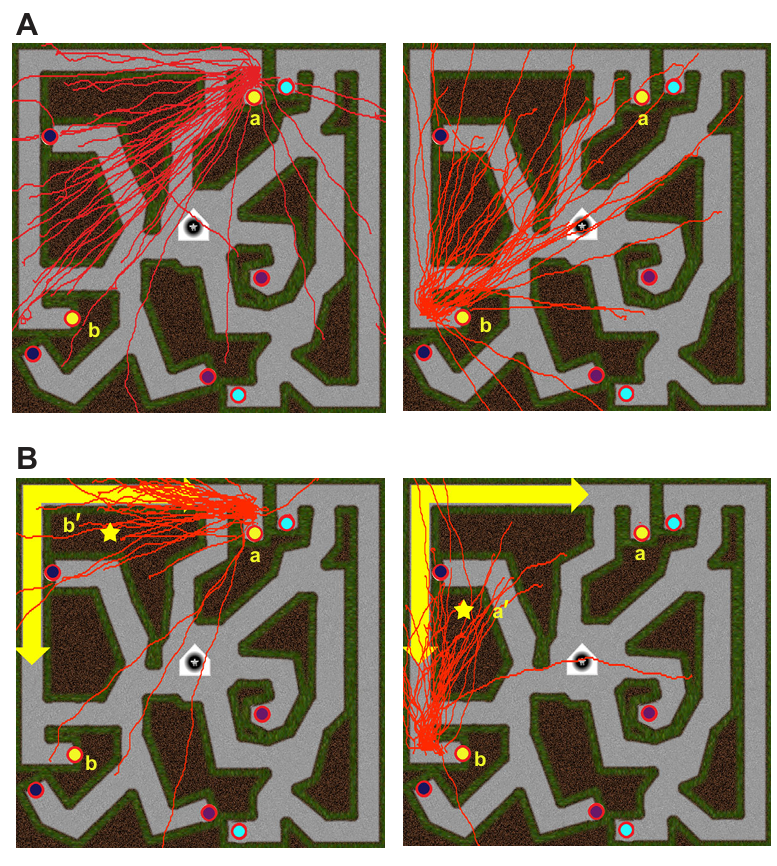
\includegraphics[width=0.45\textwidth]{NOVAthesisFiles/Images/papers/warrens-mazes-paths.png}
    \caption[Paths users took in study by Warren]{Paths taken between objects Bookcase and Cactus in Euclidean maze A and Non-Euclidean maze B. 
    Stars in maze B indicate the location of the object in Non-Euclidean coordinates. The dense amount of paths in the direction of these 
    stars show that participants' Wayfinding was highly biased by the Wormholes.~\cite{Warren2019}}
    \label{fig:warrens-mazes-paths}
\end{figure}
With this demonstration, it is conclusive that Non-Euclidean Spaces are primed for \gls{VR} use. In the next sections, the advantages that this 
type of spaces have for \gls{RDW} will be explored.

\subsection{Impossible Spaces}
\label{sec:impossible-spaces}

Fictional works such as the science-fiction TV show from BBC \textit{Doctor Who} include spaces that defy the physical laws of our reality, 
such as the TARDIS, the iconic spaceship that is "bigger on the inside", to increase the sense of wonder in their narratives. 
It was not long after the "second-wave of \gls{VR} development"~\cite{Anthes2016} that fans of the show tried to recreate this feeling of 
wonderment by bringing the famous police box to life through the use of \gls{VR}, due to its immersive capabilities
\footnote{TARDIS VR by itch.io user \textit{feroxxy} - \href{https://feroxxy.itch.io/tardisvr}{https://feroxxy.itch.io/tardisvr} - Last Access: Jan 2025 } 
. This project and the previously mentioned study by Warren~\cite{Warren2019} are prime examples of what Impossible Spaces are and their 
general application in \gls{VR}

\begin{figure}[b]
    \centering
    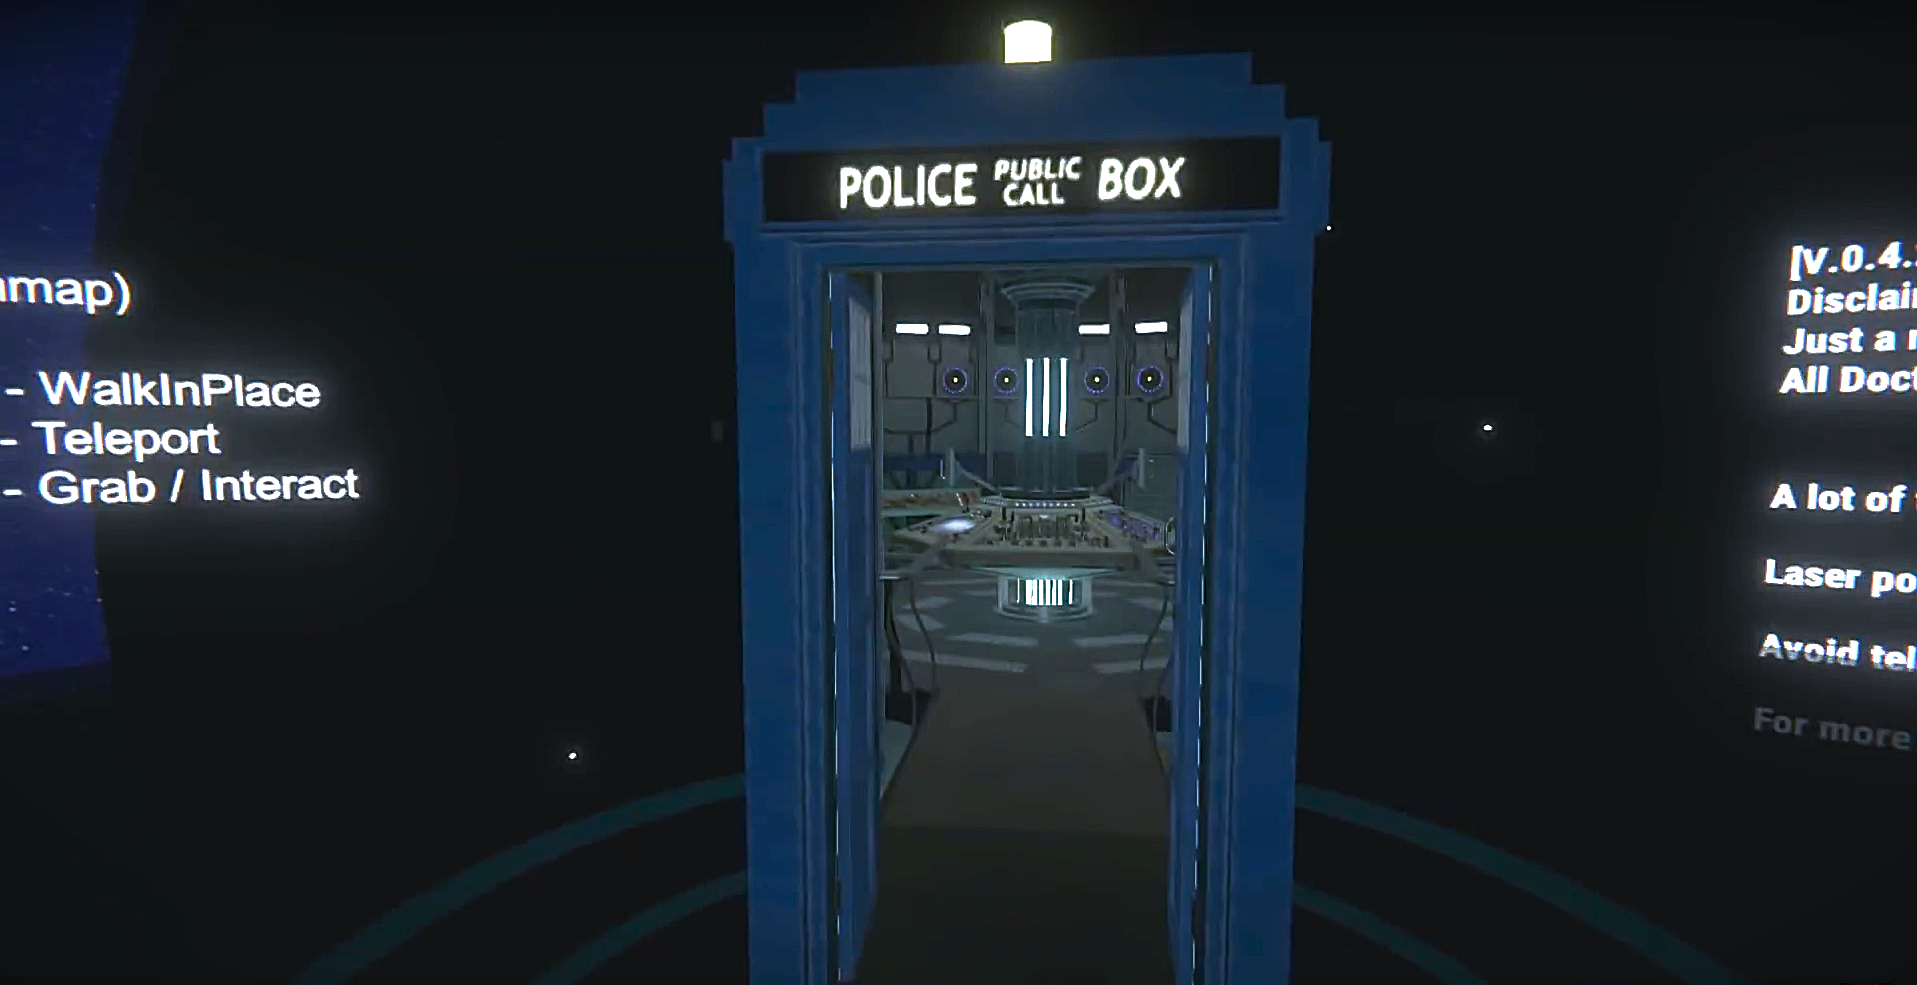
\includegraphics[width=0.85\textwidth]{NOVAthesisFiles/Images/papers/tardis.png}
    \caption[Screenshot of the TARDIS VR project]{A screenshot of the TARDIS VR project, depicting the famous police box that is "bigger on the inside", one of the possible ways to 
    depict an Impossible Space in \gls{VR}.}
    \label{fig:tardis}
\end{figure}

Impossible Spaces are, in the majority of cases~\cite{Lochner2021}, experiences taking place in \glspl{VE} that violate the rules of Euclidean 
Space, yet keep the appearance of the real world by keeping most of its Euclidean Geometry intact. This creates large \glspl{VE} that are essentially 
multiple Euclidean spaces that look ordinary when experienced locally, but when their topology is inspected, it is clear that
these spaces are connected in a manner that is physically impossible. This creates the often called "Self-Overlapping Architectures"~\cite{Lochner2021, Suma2012}.

These \glspl{VE} capitalize on the lack of physical restrictions to create an architecture that fits within physical tracking spaces,
granting users the ability to naturally walk in a much larger \gls{VE} by
redirecting users away from the edges of their tracking space~\cite{Fisher2017, Suma2012, 6550194}, 
hence the use of Impossible Spaces is considered a form of \gls{RDW}~\cite{8255772}.
Given that \gls{RDW} is a highly immersive method of locomotion, due to the walking motion it employs, 
as seen in the previous \nameref{sec:redirected-walking} section, 
in conjunction with the fact that users perceive the local environment as a Euclidean space, since distance 
perception is accurate by norm~\cite{Barwulor2020}, Impossible Spaces provide a highly immersive \gls{VR} experience. 

The illusion of the self-overlapping architecture is mostly unnoticeable, especially when users are naive to the manipulation at hand 
~\cite{Suma2012}. Distractors, visual and auditory feedback, and contextual environmental events are potential auxiliary methods to 
raise the \gls{VE}'s level of immersion~\cite{Ciumedean2020,Fisher2017}, since these methods help lower the overtness of the redirection that is 
taking place.

\gls{VR} applications typically use two main methods to connect the various sections of a Self-Overlapping Architecture: 

\begin{itemize}

    \item \textbf{Transitioning Areas} - Transitional spaces that link different sections by recurring to the previously discussed 
    "change blindness" redirection technique. These areas are usually curved corridors that restrict users' \gls{FOV}, 
    allowing for the mentioned changes to happen without the users' knowledge~\cite{5759455, Vasylevska2017} (Figure~\ref{fig:transioning-areas}).
    
    \item \textbf{Portals} - As discussed in the \nameref{sec:redirected-walking} section, \todo{portals estão agora está expandidos numa secção}
    the instantaneous teleportation caused by Overt Discrete Repositioning \gls{RDW} techniques could be highly disorienting if the user is 
    not prepared or does not have the context for such repositioning. Portals help mitigate the overtness of this technique, serving as preview 
    to the location the user is going to teleport to after passing through it~\cite{Freitag2014}. The transition between the locations can 
    be seamless, such as the wormholes from the previously mentioned study by William Warren~\cite{Warren2019}, 
    making the teleportation even less noticeable, and therefore, more immersive. 
    The "Non-Euclidean Worlds Engine" project 
    \footnote{Video on the "Non-Euclidean Worlds Engine" by \textit{Code Parade} - \href{https://youtu.be/kEB11PQ9Eo8}{https://youtu.be/kEB11PQ9Eo8} - Last Access: Jan 2025 }
    provides several examples in which these portals might be used (Figure~\ref{fig:self-Overlapping}).

\end{itemize}

\begin{figure}[b]
    \centering
    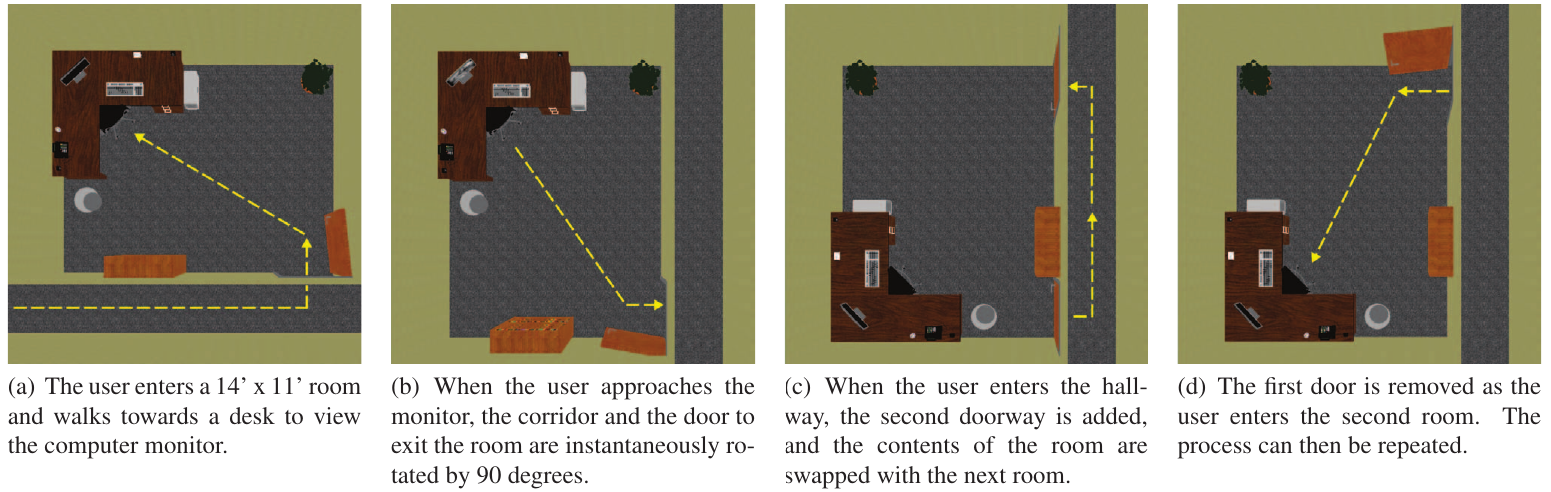
\includegraphics[width=\textwidth]{NOVAthesisFiles/Images/papers/transioning-areas.png}
    \caption[Possible implementation of change-blindness redirection]
    {A step-by-step explanation of a possible implementation of change blindness redirection through the use of a Transitioning Area. 
   ~\cite{5759455}}
    \label{fig:transioning-areas}
\end{figure}

\begin{figure}[t]
   \centering
    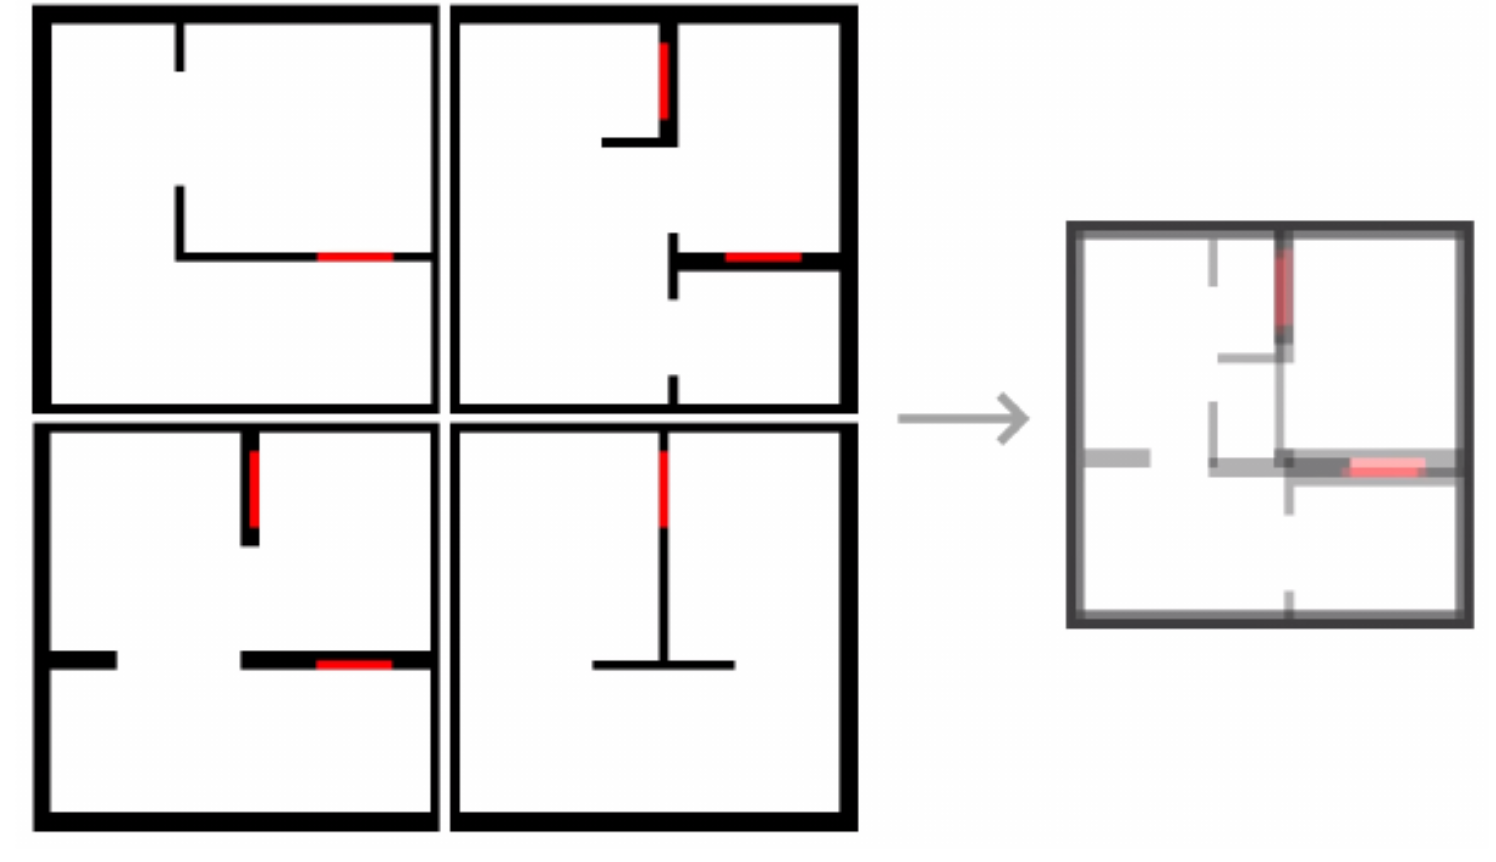
\includegraphics[width=0.5\textwidth]{NOVAthesisFiles/Images/papers/self-overlapping.png}
    \caption[Illustration of a Self-Overlapping Architecture]{A visual representation of a self-overlapping architecture from the "Non-Euclidean Worlds Engine" project.
    The four separate rooms (left) are merged together (right) through the use of portals represented in red, compressing them into a 
    \gls{VE} that only requires a physical space four times smaller than the one occupied by the four rooms.}
   \label{fig:self-Overlapping}
\end{figure}

The use of Impossible Spaces presents as a solution to map a large \gls{VE} into a limited physical tracking space, and its applications 
with \gls{RDW} techniques seem to be extensive, all depending on the context and needs the \gls{VR} application is being developed.
Flexible Spaces, developed by Vasylevska et al.~\cite{6550194}, serves as an example of how extensive these possibilities can be,
as it is a combination of the mentioned techniques, that in conjunction with \textit{Procedural Content Generations}, 
creates an all-in-one dynamically adjustable redirection technique. 


\subsection{Portals}
\label{sec:portals}

As discussed in Section \ref{sec:redirected-walking}, the instantaneous teleportation caused by Overt Discrete Repositioning 
\gls{RDW} techniques can be disorienting if users are not provided with an appropriate cue. Portals address this issue by 
acting as gateways between distant points in a self-overlapping Impossible Space, offering a preview of the connected environment 
and cueing users that they may be transported to the displayed destination by stepping through the portal~\cite{Freitag2014,Jaksties2022,Liu2018b,Lochner2021}.

\begin{figure}[b]
    \centering
     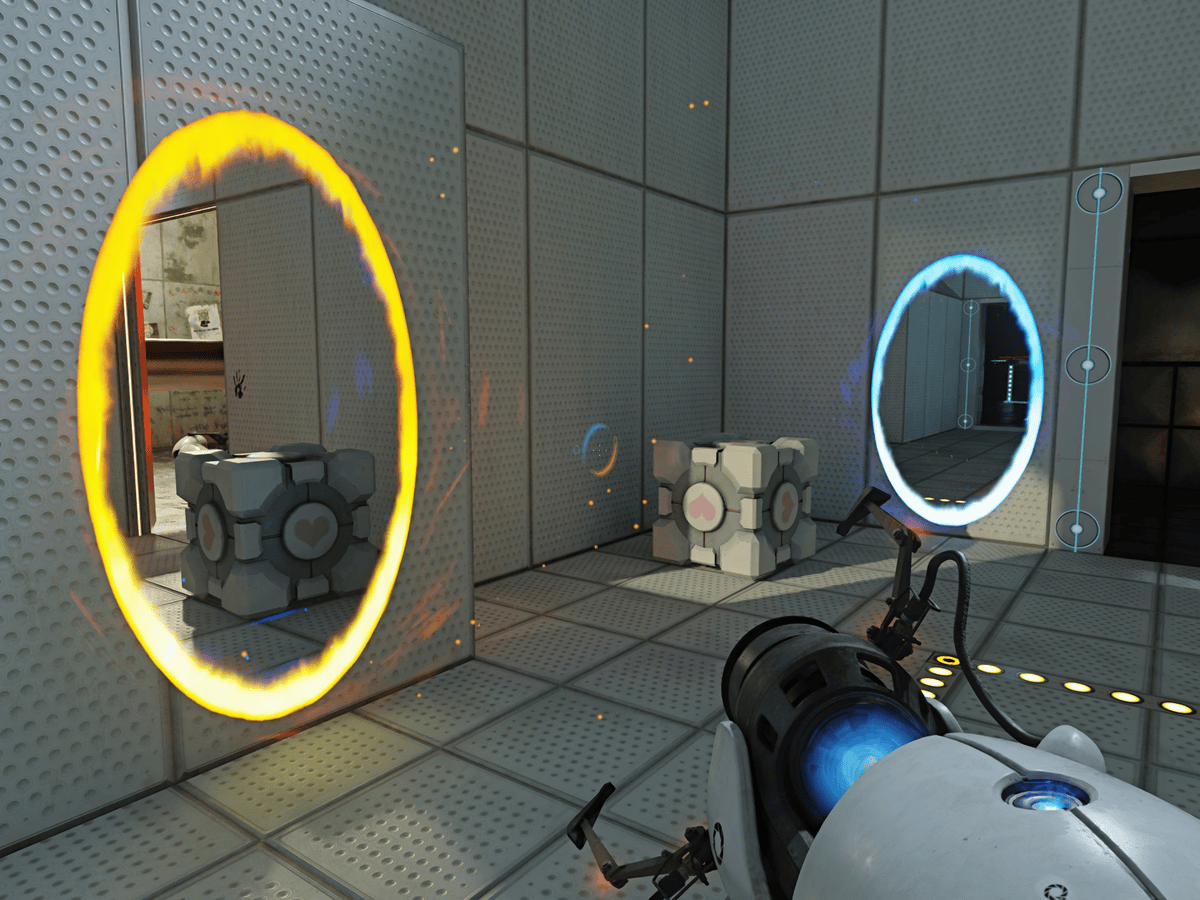
\includegraphics[width=0.5\textwidth]{NOVAthesisFiles/Images/papers/Portal-with-RTX-ultra-quality.png}
     \caption[Screenshot of the Portal video game]
     {In the video game \textit{Portal}, players must solve puzzles using a pair of connected blue and orange portals. In this example the preview 
     capabilities of portals is displayed, as it is possible to see the previews of the orange and blue portals.}
     \label{fig:portal}
\end{figure}

Portals are most prevalent in the video game scene~\cite{Murray2019}, brought to popularity by the 2007 game \textit{Portal} from 
\textit{Valve}~\footnote{Portal Steam page - \href{https://store.steampowered.com/app/400/Portal/}{https://store.steampowered.com/app/400/Portal/}, Last Access - Aug 2025 }, 
however research on the use of portals in \gls{VR} applications is still ongoing. In \gls{VR} research, various iterations of portals 
have been developed and researched for various functions, such as:

\begin{itemize}
    \item \textbf{Redirected Walking} - A common use for portals in \gls{VR} relies on their use for \gls{RDW}. 
    Comparitive works such as those by Lochner \& Gain~\cite{Lochner2021} 
    and Rebelo et al.~\cite{Rebelo2024b} recur to the use of portals as a means to compare Natural Walking locomotion using portals and 
    other means of \gls{VR} locomotion.
    Usually door-shaped, these portals connect various points in a self-overlapping Impossible Space, compressing the \gls{VE} into 
    the limited physical tracking space, allowing users to naturally walk through the environment (Figure~\ref{fig:self-Overlapping}).
    
    \item \textbf{Extended Reach} - Window-shaped portals have been used as a means to extend reach, enabling users to reach to otherwise 
    unreachable objects blocked by distance or obstacles~\cite{Han2022,Ablett2024}. Variations include the ability to move the portal in real-time~\cite{Ablett2024} 
    and having a mirroring functionality~\cite{Li2021}.
    
    
     \begin{figure}[b]
        \centering
        % First row: (a) and (b)
        \begin{subfigure}{0.4\textwidth} % Smaller width for each subfigure
            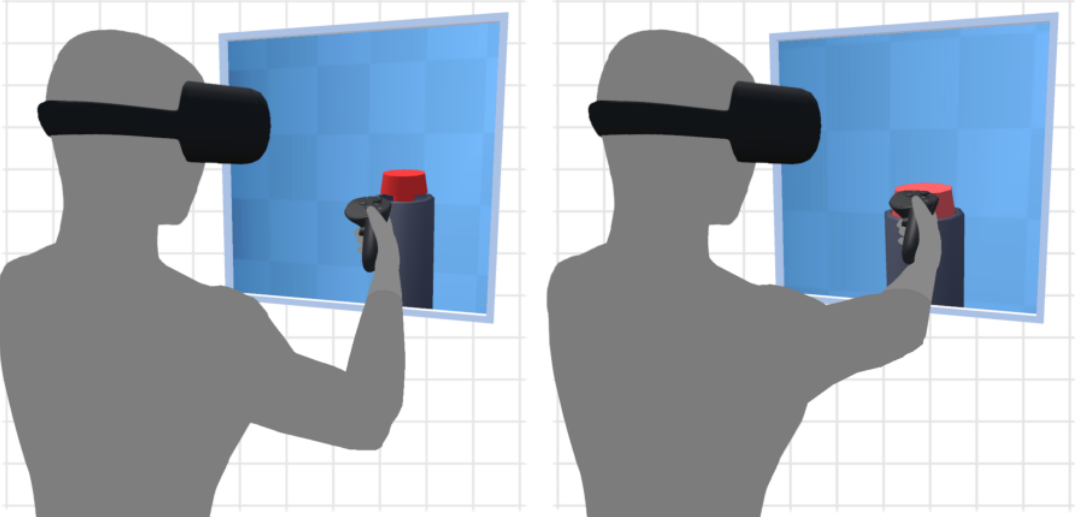
\includegraphics[width=\linewidth]{NOVAthesisFiles/Images/papers/reach.png}
            \caption{Portals may be used to extend users reach, creating a window that allows users to interact with distant objects.~\cite{Ablett2024}}
            \label{fig:avatars-torso}
        \end{subfigure}
        \begin{subfigure}{0.4\textwidth} % Smaller width for the bottom image
            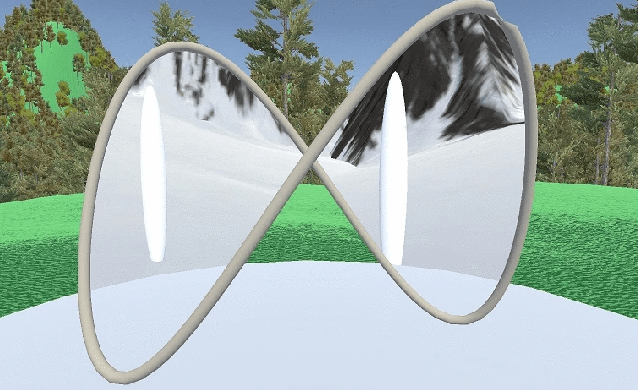
\includegraphics[width=\linewidth]{NOVAthesisFiles/Images/papers/knotted-portal.png}
            \caption{Portals may be used as a means to explore complex topological structures, such as this knotted portal.~\cite{Summermann2021}}
            \label{fig:avatars-vive-trackers}
        \end{subfigure}
        \begin{subfigure}{.8\textwidth} % Smaller width for each subfigure
            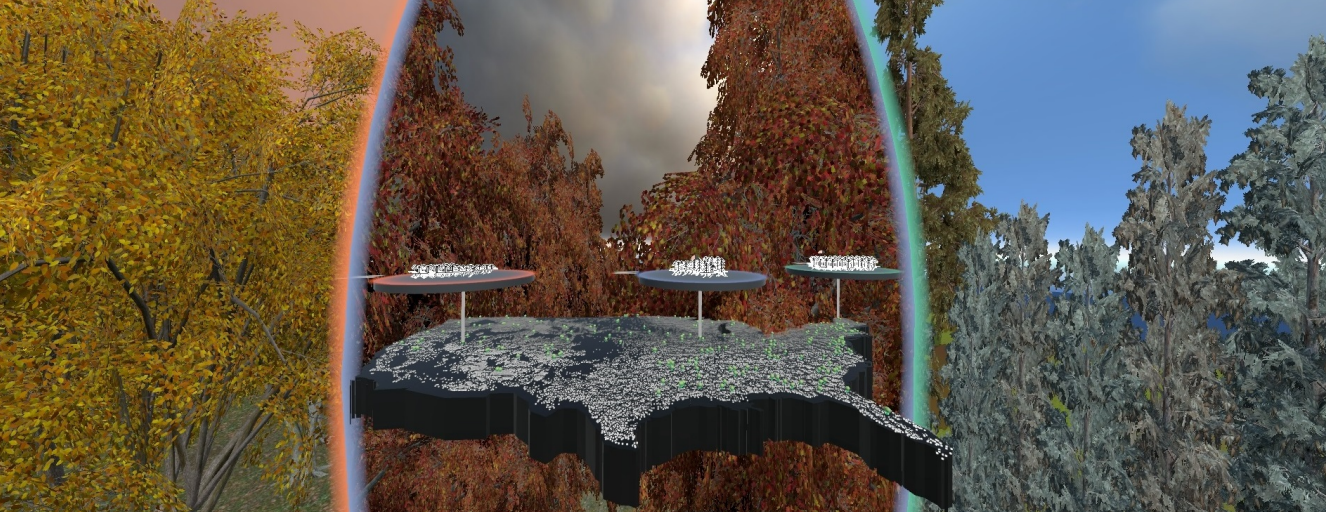
\includegraphics[width=\linewidth]{NOVAthesisFiles/Images/papers/wedge.png}
            \caption{Portals have also been used as a means to compare different worlds through juxtaposition, such as forestry data.~\cite{Nam2019}}
            \label{fig:avatars-ik-legs}
        \end{subfigure}
        \caption[Multiple portal applications in VR]{Multiple portal applications in \gls{VR}.}
        \label{fig:mappings}
    \end{figure}
    \item \textbf{Visualization/Comparison} - Portals may also be used to compare or visualize \glspl{VE} that are irreproducible in the 
    real world. This has been done through the use of volumetric wedges, that allow the comparison of multiple virtual worlds through 
    juxtaposition~\cite{Nam2019}, and the use of portals constructed from knotted curves that offer a novel way to explore complex topological 
    structures~\cite{Summermann2021}.
\end{itemize}

The aforementioned portal variants share the use of a stereoscopically rendered plane, which provides a preview of the destination 
space and enables a seamless transition from the entry to the destination portal. A common method of rendering this preview is through the use of 
stencil buffers~\cite{Murray2019}, which can be thought of as a 2-dimensional arrays that are the same size
as the user's screen. Each portal has an associated camera that is placed relatively with the user's camera and the opposing side of 
the portal, as if the user position was mirrored. Thus, both the position and rotation (and scale if the paired portals have different scales) of 
the camera must be modified accordingly. 

The rendering of a scene through the stencil buffer approach is done recursively. The buffer stores the recursion level of each pixel, corresponding 
to which level of "depth" it is (0 - user's view; 1 - portal in the user's view; 2 - portal inside a portal in the user's view; etc.). When rendering the 
frame, the algorithm goes through each recursion level, only rendering the pixels equivalent with said level with the corresponding camera. As such, 
the method starts by rendering the pixels outside a portal through the user's camera, then it renders the portal's view through the portal's camera, 
and so on for all recursion levels. Figure~\ref{fig:stencil-buffer} exemplifies a simplified version of a stencil buffer.

\begin{figure}[b]
    \centering
     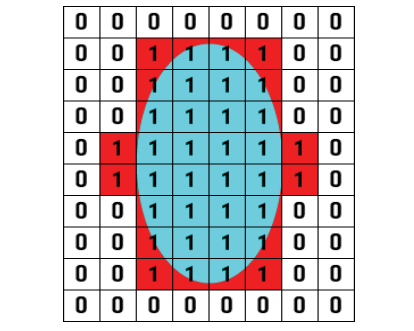
\includegraphics[width=0.6\textwidth]{NOVAthesisFiles/Images/papers/stencil buffer.png}
     \caption[Simplified representation of a stencil buffer for rendering portals.]
     {A simplified representation of a stencil buffer when rendering a portal. The inner oval contains multiple pixels with a recursion depth of 1,
     that represents the portal.}
     \label{fig:stencil-buffer}
\end{figure}


Another common approach for rendering portal views is through the use of pre-rendered textures. It involves placing the camera as described above, however, rather 
than rendering the view as the previous method does, it saves it into a texture and places the pre-rendered texture on the portal. Although a 
simpler approach, this method does not supply the same visual fidelity as through the use of stencil buffers.

A common problem for both these rendering methods may occur as the result of having objects between the portal and the camera's view, 
named the “banana juice problem”~\footnote{CS50's Introduction to Game Development 2018; Lecture 11- \href{https://youtu.be/ivyseNMVt-4}{https://youtu.be/ivyseNMVt-4}, Last Access - Aug 2025 }. 
This results in unorthodox view through the portal, solved by not including the objects when rendering, 
also known as \textit{clipping}.

\begin{figure}[t]
    \centering
     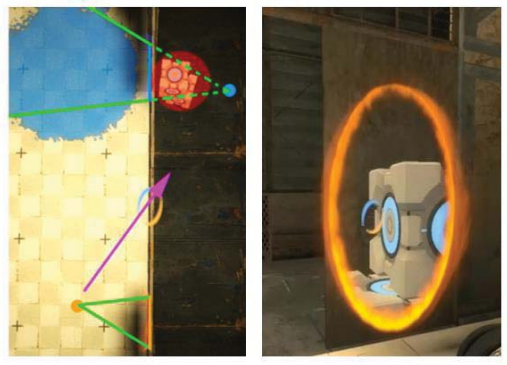
\includegraphics[width=0.75\textwidth]{NOVAthesisFiles/Images/papers/banana-juice.png}
     \caption[Example of the 'banana juice problem'.]
     {The "banana juice problem" occurs when there are objects between a portal and its associated camera for rendering the preview.
     To solve this issue, the camera must clip(not render) any of the objects or structures between the camera and the portal.~\cite{Murray2019}}
     \label{fig:banana-juice}
\end{figure}

\subsection{Hyperbolic Spaces}
\label{sec:hyperbolic-spaces}

\todo{Hyperbolic Spaces acabaram por não serem utilizados. Vale a pena manter esta subsecção para contexto no trabalho preliminar?}

As stated before, Non-Euclidean Geometry is a variant of Euclidean Geometry by having its axioms changed, one of them 
being Euclid's Parallel Postulate.
It states that through any given point not on a line there passes exactly one line parallel to that line in the same plane~\cite{Eryk2018}. 
If one were to change this axiom to either permitting the existence of two or more parallel lines or restricting it to no parallel lines, 
they would get Hyperbolic and Elliptic Spaces, respectively~\cite{Pisani2019}.

Hyperbolic Spaces are then infinite by definition, having more space available in a given distance than in Euclidean Spaces, presenting a 
constant negative curvature~\cite{Pisani2019}. Its properties make it valuable for the representation of relational data, as its infinity allows 
integrating trees of data with deliberately large sizes, proving more useful than Euclidean Graphs~\cite{Eryk2017, Liu2019}. 
An example of this is the hyperbolic graph of most used languages in GitHub, created by Celiska et al.~\cite{Celiska2017} and represented in 
Figure~\ref{fig:github}, 
in which the distances between the language nodes indicated how frequently these programming languages were used together.

\begin{figure}[t]
    \centering
     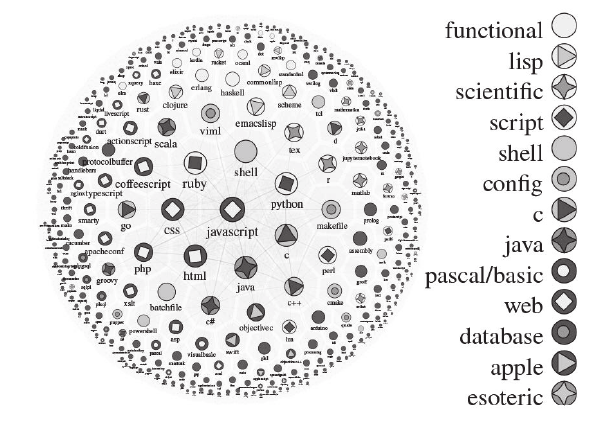
\includegraphics[width=0.6\textwidth]{NOVAthesisFiles/Images/papers/github.png}
     \caption[Hyperbolic graph of GitHub's most used languages]{Hyperbolic graph of GitHub's most used languages. The closer the language nodes are, the more frequently these 
     languages are used together.~\cite{Celiska2017}}
    \label{fig:github}
 \end{figure}

 \begin{figure}[b]
     \centering
      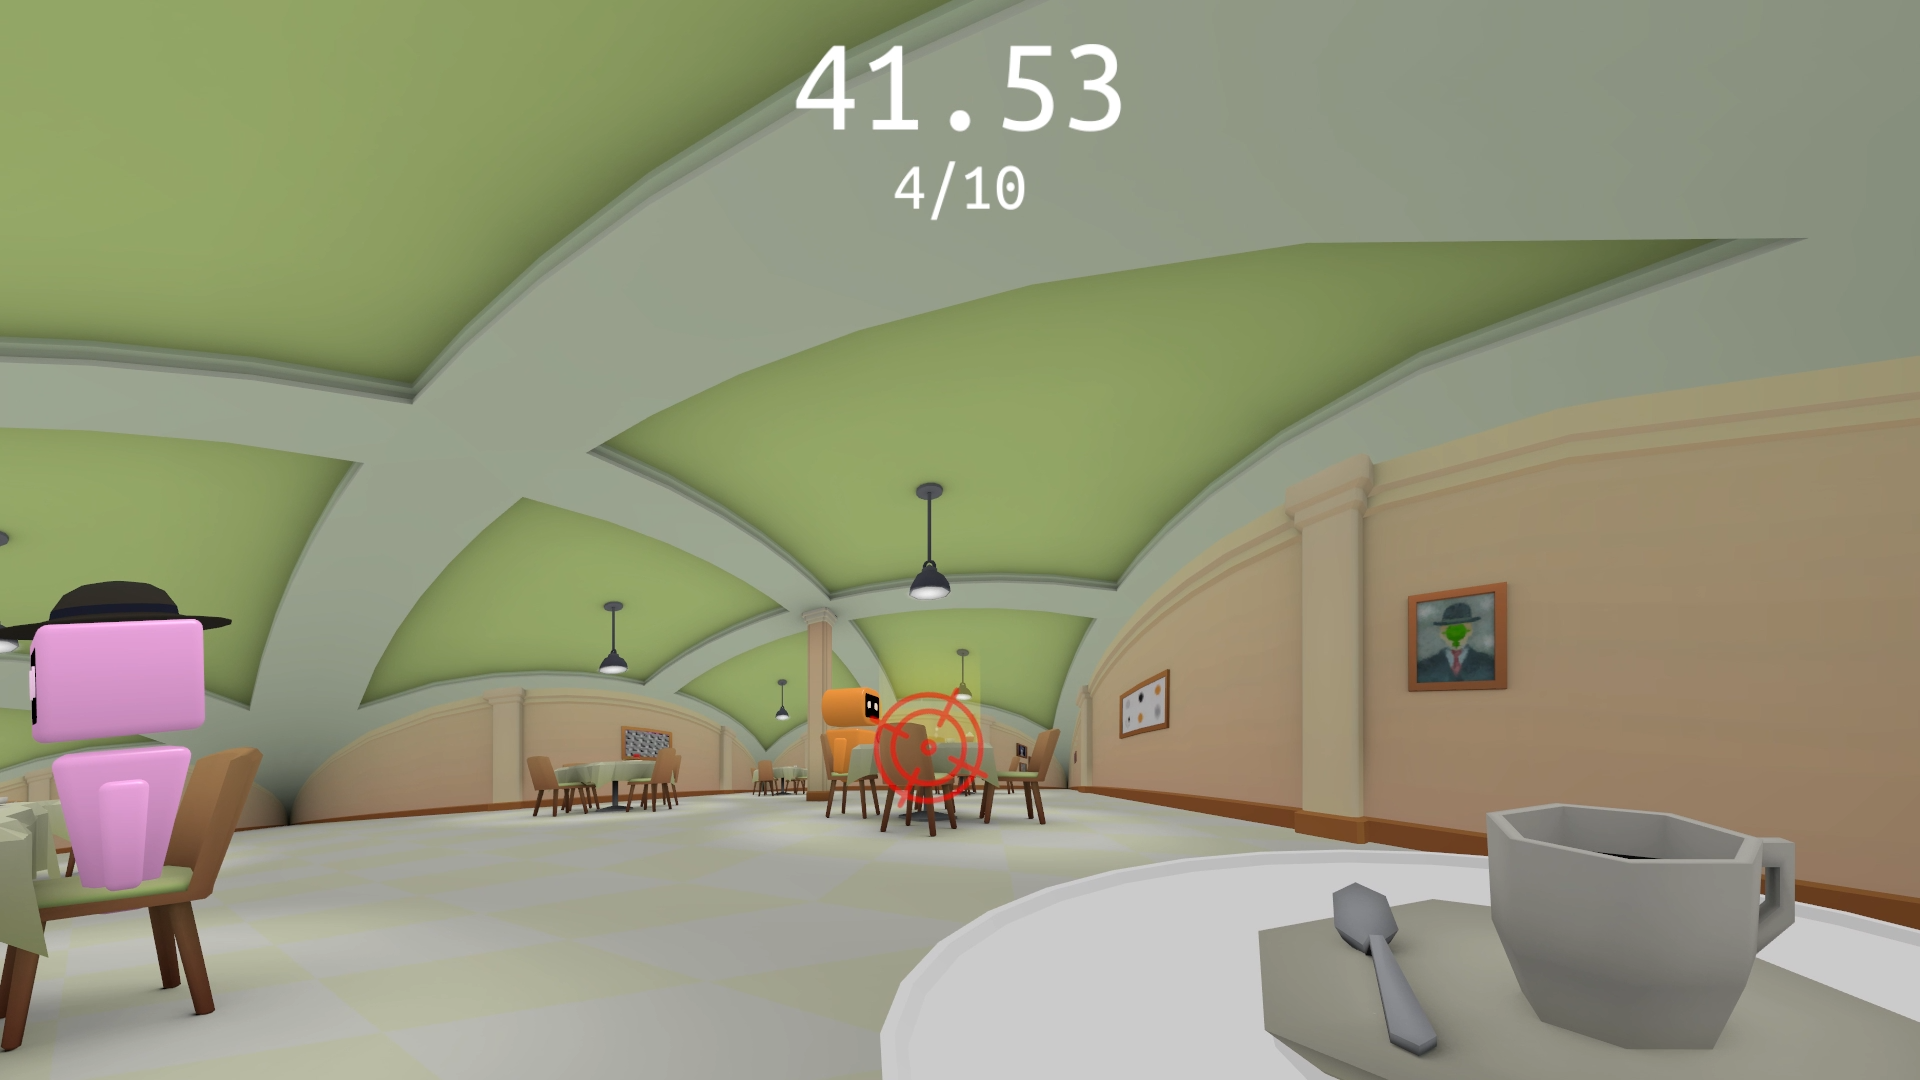
\includegraphics[width=0.75\textwidth]{NOVAthesisFiles/Images/papers/hyperbolica.png}
      \caption[Screenshot of one of the levels from the game Hyperbolica.]{A screenshot of one of the levels from the game Hyperbolica.}
     \label{fig:hyperbolica}
  \end{figure} 

Entertainment has also benefited from Hyperbolic Geometry in the video-game industry, as games like \textit{Hyperbolica} (Figure~\ref{fig:hyperbolica})
\footnote{Hyperbolica Steam page - \href{https://store.steampowered.com/app/1256230/Hyperbolica/}{https://store.steampowered.com/app/1256230/Hyperbolica/}, Last Access - Jan 2025 } 
and \textit{HyperRogue}~\cite{Eryk2017}
have integrated hyperbolic spaces into their gameplay to create challenging puzzles and situations for players to solve. 
With the seamless integration of Hyperbolic Spaces in video games, 
it could be reasonable to assume that these would translate well into \gls{VR}. The literature on the matter, although not complete, 
is extensive enough to confirm that there is an interest in researching this topic.


The visual tool by Hart et al.~\cite{Hart2017} is an example on this interest, as they aimed to create a \gls{VR} experience that allows users to 
more intuitively grasp Hyperbolic Geometry. Various models were used to simulate this space, and the application permitted users to navigate through 
the \gls{VE}, which proved a challenge. Due to the space's negative curvature, phenomena as \textit{holonomy} - 
a result of parallel transporting vectors along a closed loop - occurs, which can make Hyperbolic Spaces highly disorienting, 
since it translates into effects, such as the floor appearing to move away 
or rotate. Authors purposed methods of solving this issue, though they were recognized as artificial means that "hack" the simulation.

Rebelo et al.~\cite{Rebelo2022} have also conducted research on the use of Hyperbolic Spaces in \gls{VR}. One of the studies conducted in this work 
pretended to examine how users would react to different mappings between virtual and physical spaces, using tangible objects on a table that users 
had to move and rotate. The four different mappings (Figure~\ref{fig:mappings}) were either mapped by linear functions - correspondent to Euclidean Spaces - 
or Hyperbolic functions - correspondent to the Non-Euclidean Spaces - in this case the hyperbolic tangent and its inverse, morphing space so that 
the center of the table occupied more or less space, respectively. Results revealed that 
there were no significant differences in terms of efficiency between two linear and hyperbolic scenarios, and the research concluded that users 
were able to adapt do Hyperbolic Spaces quickly, going in accordance with the previously mentioned work from Hart et al.~\cite{Hart2017} and 
study by Pisani et al.~\cite{Pisani2019}

 \begin{figure}[t]
    \centering
    % First row: (a) and (b)
    \begin{subfigure}{0.45\textwidth} % Smaller width for each subfigure
        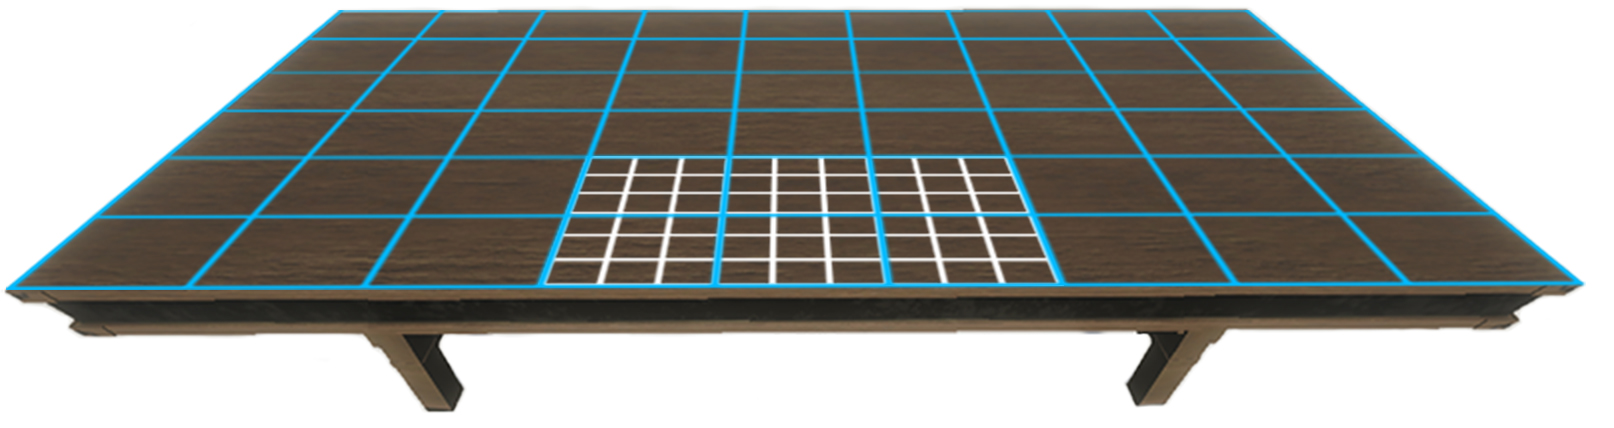
\includegraphics[width=\linewidth]{NOVAthesisFiles/Images/papers/table-linear.jpg}
        \caption{The resultant mappings of linear functions: \(x\) for white and \(3x\) for blue lines.}
        \label{fig:avatars-torso}
    \end{subfigure}
    \begin{subfigure}{0.45\textwidth} % Smaller width for each subfigure
        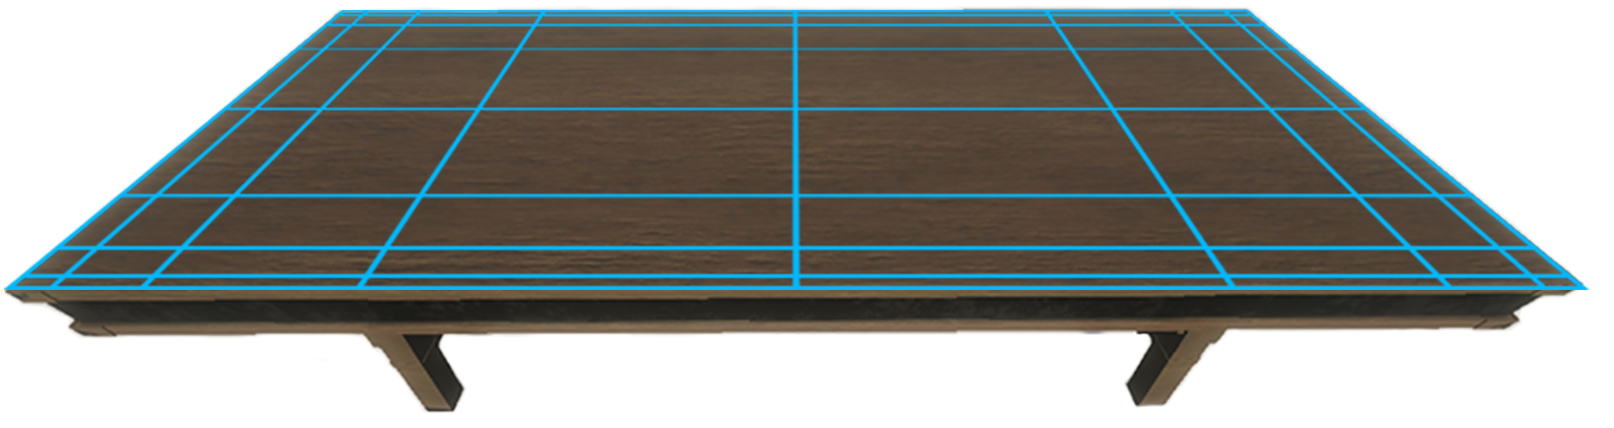
\includegraphics[width=\linewidth]{NOVAthesisFiles/Images/papers/table-hyperbolic1.jpg}
        \caption{The resultant mapping of the hyperbolic tangent function (\textit{tanh}).}
        \label{fig:avatars-ik-legs}
    \end{subfigure}
    \begin{subfigure}{0.45\textwidth} % Smaller width for the bottom image
        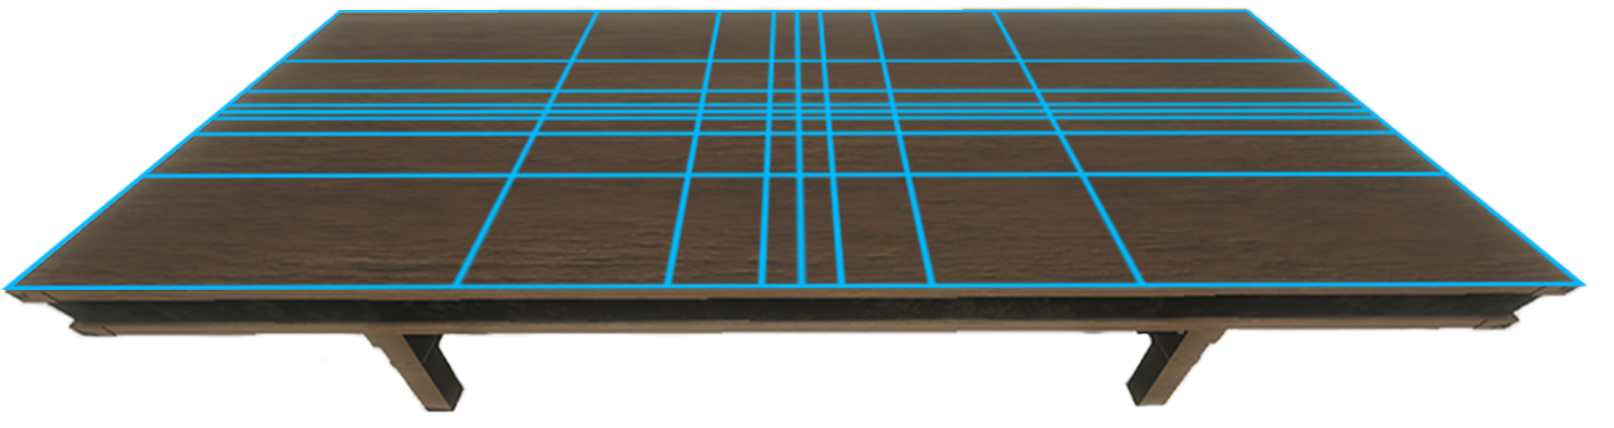
\includegraphics[width=\linewidth]{NOVAthesisFiles/Images/papers/table-hyperbolic2.jpg}
        \caption{The resultant mapping of the inverse hyperbolic tangent function (\textit{arctanh}).}
        \label{fig:avatars-vive-trackers}
    \end{subfigure}
    \caption[Mappings by Rebelo et al.]{The four mappings studied by Rebelo et al. \cite{Rebelo2022}}
    \label{fig:mappings}
\end{figure}
  

 %The work by Rebelo et al.~\cite{Rebelo2022} additionally mentions the existence of a gap in research on the use of Hyperbolic Spaces in \gls{VR} applications, which 
 %is arguably still felt, particularly on the navigation of \glspl{VE} with large interiors. Our work pretends to fill this gap, by integrating a 
 %similar implementation of Hyperbolic Space mapping to test the feasibility of using these Non-Euclidean Spaces for navigation in \gls{VR}.

 \section{Summary}
\label{sec:summary}

In summary, this chapter has introduced concepts of \gls{VR}, and how \glspl{VE} are constructed and navigated, in order to have the base context 
of what locomotion techniques are and how they affect \gls{VR} navigation. 

As such, various locomotion techniques were explored, addressing how 
their characteristics differ from each other and hence have different strong points and limitations. Since the objective of this work is to 
contribute to immersive navigation, it was concluded that \gls{RDW} techniques were the most indicated, as these techniques employ continuous 
motion through natural walking, achieving higher feelings of presence in the \gls{VE}, compared to other techniques.

The limitations of \gls{RDW} were also addressed, as naturally walking in a constricted physical space is still a challenge in the 
implementation of these techniques. Our work addresses this challenge by employing redirection through the use of non-Euclidean \glspl{VE}, 
thus non-Euclidean geometry and its applications in \gls{VR} have been explored in this chapter as well. The particular examples of 
non-Euclidean spaces explored were Impossible and Hyperbolic Spaces, as these allow natural walking in large \glspl{VE} whilst in limited 
tracking spaces.